%%%%%%%%%%%%%%%%%%%%%%%%%%%%%%%%%%%%%%%%%
% American Geophysical Union (AGU)
% LaTeX Template
% Version 1.0 (3/6/13)
%
% This template has been downloaded from:
% http://www.LaTeXTemplates.com
%
% Original author:
% The AGUTeX class and agu-ps referencing style were created and are owned
% by AGU: http://publications.agu.org/author-resource-center/author-guide/latex-formatting-toolkit/
%
% This template has been modified from the blank AGU template to include
% examples of how to insert content and drastically change commenting. The
% structural integrity is maintained as in the original blank template.
%
% Important notes:
% This template retains extensive commenting from the AGU template. It is heavily
% advised you read these comments and follow them in order to insure a speedy
% submission process.
%
%%%%%%%%%%%%%%%%%%%%%%%%%%%%%%%%%%%%%%%%%

%%%%%%%%%%%%%%%%%%%%%%%%%%%%%%%%%%%%%%%%%%%%%%%%%%%%%%%%%%%%%%%%%%%%%%%%%%%%
% AGUtmpl.tex: this template file is for articles formatted with LaTeX2e,
% Modified March 2013
%
% This template includes commands and instructions
% given in the order necessary to produce a final output that will
% satisfy AGU requirements.
%
% PLEASE DO NOT USE YOUR OWN MACROS
% DO NOT USE \newcommand, \renewcommand, or \def.
%
% FOR FIGURES, DO NOT USE \psfrag or \subfigure.
%
%%%%%%%%%%%%%%%%%%%%%%%%%%%%%%%%%%%%%%%%%%%%%%%%%%%%%%%%%%%%%%%%%%%%%%%%%%%%
%
% All questions should be e-mailed to latex@agu.org.
%
%%%%%%%%%%%%%%%%%%%%%%%%%%%%%%%%%%%%%%%%%%%%%%%%%%%%%%%%%%%%%%%%%%%%%%%%%%%%

% Step 1: Set the \documentclass

% There are two options for article format: two column (default) and draft.

% PLEASE USE THE DRAFT OPTION TO SUBMIT YOUR PAPERS.
% The draft option produces double spaced output.

% Choose the journal abbreviation for the journal you are submitting to:

% jgrga	JOURNAL OF GEOPHYSICAL RESEARCH
% gbc	GLOBAL BIOCHEMICAL CYCLES
% grl		GEOPHYSICAL RESEARCH LETTERS
% pal	PALEOCEANOGRAPHY
% ras	RADIO SCIENCE
% rog	REVIEWS OF GEOPHYSICS
% tec	TECTONICS
% wrr	WATER RESOURCES RESEARCH
% gc		GEOCHEMISTRY, GEOPHYSICS, GEOSYSTEMS
% sw	SPACE WEATHER
% ms	JAMES
%
%
%
% (If you are submitting to a journal other than jgrga,
% substitute the initials of the journal for "jgrga" below.)

\documentclass[draft, jgrga]{AGUTeX}

% can I use these symbols?
\usepackage{array,amssymb}

% permil symbol
\usepackage{ wasysym }

% To create numbered lines:

% If you don't already have lineno.sty, you can download it from http://www.ctan.org/tex-archive/macros/latex/contrib/ednotes/ (or search the internet for lineno.sty ctan), available at TeX Archive Network (CTAN). Take care that you always use the latest version.

% To activate the commands, uncomment \usepackage{lineno} and \linenumbers*[1]command, below:

%\usepackage{lineno}
%\linenumbers*[1]

%  To add line numbers to lines with equations:
%  \begin{linenomath*}
%  \begin{equation}
%  \end{equation}
%  \end{linenomath*}

%%%%%%%%%%%%%%%%%%%%%%%%%%%%%%%%%%%%%%%%%%%%%%%%%%%%%%%%%%%%%%%%%%%%%%%%%
% Figures and Tables

% DO NOT USE \psfrag or \subfigure commands.

%  Figures and tables should be placed AT THE END OF THE ARTICLE, after the references.

%  Uncomment the following command to include .eps files (comment out this line for draft format):
%\usepackage[dvips]{graphicx}
\usepackage{graphicx}
\usepackage{caption}
%\usepackage{subfig}


% Substitute one of the following for [dvips] above if you are using a different driver program and want to proof your illustrations on your machine:
% [xdvi], [dvipdf], [dvipsone], [dviwindo], [emtex], [dviwin],
% [pctexps],  [pctexwin],  [pctexhp],  [pctex32], [truetex], [tcidvi],
% [oztex], [textures]

%  Uncomment the following command to allow illustrations to print when using Draft:
\setkeys{Gin}{draft=false}

% See how to enter figures and tables at the end of the article, after references.

%----------------------------------------------------------------------------------------
%	RUNNING HEAD AND CORRESPONDING AUTHOR
%----------------------------------------------------------------------------------------

% Author names in capital letters:
\authorrunninghead{Authors}

%------------------------------------------------

% Shorter version of title entered in capital letters:
\titlerunninghead{CFA DATA DIFFUSION LENGTHS}

%------------------------------------------------

% Corresponding author mailing address and e-mail address:
\authoraddr{Corresponding author: Emma Kahle, Earth and Space Sciences Department, University of Washington, Seattle, WA, USA. (eckahle@uw.edu)}

%----------------------------------------------------------------------------------------

\begin{document}

%----------------------------------------------------------------------------------------
%	TITLE
%----------------------------------------------------------------------------------------

\title{Estimating diffusion lengths of water isotopes from ice core data measured by continuous flow analysis}

%----------------------------------------------------------------------------------------
%	AUTHORS AND AFFILIATIONS
%----------------------------------------------------------------------------------------

% Use \author{\altaffilmark{}} and \altaffiltext{}

% \altaffilmark will produce footnote; matching \altaffiltext will appear at bottom of page.

\authors{Emma Kahle,\altaffilmark{1}
Christian Holme,\altaffilmark{2}, and
everyone else}

\altaffiltext{1}{Department of Earth and Space Sciences, University of Washington, Seattle, Washington, USA.}

\altaffiltext{2}{CIC}

%----------------------------------------------------------------------------------------
%	ABSTRACT
%----------------------------------------------------------------------------------------

% Do NOT include any \begin...\end commands within the body of the abstract.

\begin{abstract}

We examine high-resolution water isotope data sets from continous flow analysis (CFA) of the West Antarctic Ice Sheet (WAIS) Divide (WDC) and South Pole (SPC) ice cores. Spectral analysis of water isotope data reveals damping of high-frequency variations associated with diffusive smoothing of the isotopic profile in the firn layer of an ice sheet. This diffusion of water isotope ratios in ice cores can provide information about past firn conditions. The data spectra of windowed sections of CFA data from WDC and SPC show different characteristics as compared with similar discretely-sampled data sets, affecting the estimation of high-frequency damping due to the firn diffusion process. The cause of this spectral difference is not known, but we suggest possible explanations in the CFA measurement system and in natural firn proceses. Without knowing the origin of this spectral difference, we can still parameterize a method to estimate the extent of diffusion in the spectra. In this study we use two modified techniques to estimate extent of diffusion in order to efficiently and accurately produce diffusion estimates for full ice core CFA data sets.

\end{abstract}

%----------------------------------------------------------------------------------------
%	ARTICLE CONTENT
%----------------------------------------------------------------------------------------

% The body of the article must start with a \begin{article} command
% \end{article} must follow the references section, before the figures and tables.

\begin{article}

\section{Introduction}

To understand past and future climate change, water isotope data from ice cores have long been used as climate proxies, based on the temperature-dependent distillation of water isotope ratios (e.g. $\delta^{18}\mathrm{O}$) in the atmosphere (cite papers). This indirect method for obtaining temperature records through past glacial and interglacial cycles relies on empirical correlations that only approximate the physical processes involved. A more direct approach uses the signal of isotope diffusion preserved in the ice, overcoming the many issues related to conventional
isotope ratios \citep{Johnsen2000}.

\subsection{Stable Water Isotope Diffusion}

Water isotope diffusion occurs primarily in the firn layer, snowfall in the upper tens of meters of an ice sheet that has yet to be fully compressed into ice. As firn is permeable, water molecules can diffuse through in the vapor phase, damping the seasonal variations and high-frequency noise of the original isotope signal. As the diffusion process depends on temperature, a temperature record can be obtained by measuring the extent of diffusion that has occurred. This method is independent of conventional assumptions about isotope fractionation before deposition, and thus improves on conventional ice core temperature methods. Beyond information about past temperature, diffusion estimates also provide constraints on past firn conditions and total ice thinning. With these motivations, estimations of diffusion have been made for ice cores in both Greenland and Antarctica \citep{Johnsen2000,Simonsen2011,Gkinis2014,Jones2016}.

\subsection{Continuous Flow Analysis}

In the past, most ice core water isotope data have been measured discretely by melting vertical sections of the core. The isotope ratio of each discrete sample is measured on mass spectrometer or laser spectrometer. Recently, ice core water isotope measurements are often measured on continuous flow analysis (CFA) systems. These systems continously feed the water stable isotopes of the melting core directly into a laser spectrometer, yielding high resolution data more easily than a discrete measurement process. Depending on the amount of effort committed, discrete analyses can produce results ranging from one-meter for entire ice cores to 2.5-cm resolution for smaller sections of ice cores. Meanwhile, CFA analyses can easily produce results at half-cm resolution for an entire ice core record. This higher resolution greatly improves the ability to analyze diffusion lengths, which depend on information in the high frequencies of the data spectrum.

A number of studies have estimated diffusion lengths from discretely sampled water isotopes (\citep{Johnsen2000,Simonsen2011,Gkinis2014,VanderWel2015}). While data spectra from discrete data match well with spectra from theoretically derived synthetic data \citep{Holme2017}, spectra from CFA data have an additional characteristic in the mid-frequency range ($5^{-1}$ to $10^{-1}$ cm$^{-1}$). Figure \ref{spectra_disVScfa} demonstrates this difference by comparing the power spectra of discretely and continuously measured data. The CFA data spectra have a transition zone of sloping red noise from the damped frequencies into the system noise. The highest resolution discretely-sampled data sets do not show this transition zone in the spectrum.

Since estimating diffusion length depends on the shape of the spectrum, the presence of this transition can affect diffusion results. In this paper we describe how to estimate diffusion lengths on CFA data without the effect of this transition. We start from the approaches developed in \citet{Johnsen2000} and \citet{Gkinis2014} and propose two adjusted techniques to accommodate CFA water isotope data.

\subsection{Water Isotope Data}

We use data from the WAIS Divide and South Pole ice cores, both measured at the Institute of Arctic and Alpine Research (INSTAAR) at the University of Colorado. INSTAAR uses a CFA system to measure the water isotope ratios of $\delta^{18}\mathrm{O}$, $\delta^{17}\mathrm{O}$, and $\delta\mathrm{D}$ at a resolution of half-cm. For complete details on the INSTAAR CFA system, see \citet{JonesCFA2016}. Other published discrete and continuous water isotope data sets from Greenland and Antarctic cores were compiled for comparison.

%------------------------------------------------

\section{Diffusion Theory}

The fundamental physics of advection and diffusion can describe mathematically the post-depositional effects on the profile of water isotopes in the ice core. The majority of water isotope diffusion occurs in the firn layer where interconnected air pathways allow water vapor to diffuse vertically through the firn column. After firn densification has sealed off bubbles in the ice, vapor diffusion ceases and solid ice diffusion takes over. The process in solid ice has a diffusivity orders of magnitude smaller than that of vapor diffusion, and we do not consider it in this study.

The isotopic profile changes through the firn layer of an ice sheet due to the effects of diffusion across isotopic gradients and due to densification of the firn. As stated by \citet{Johnsen1977} and subsequently used in several diffusion studies (\citep{Johnsen2000, Simonsen2011, Gkinis2014, VanderWel2015, Jones2016, Holme2017}), these changes to the isotopic profile can be described by Fick's second law, the basic advection-diffusion equation:
\begin{equation}
\frac{\partial \delta}{\partial t}
= D \frac{\partial ^2 \delta}{\partial z^2}
- \dot{\epsilon}
z \frac{\partial \delta}{\partial z}
\end{equation}

where \begin{math} \delta \end{math} is the isotope ratio, \begin{math} D \end{math} is the diffusivity coefficient, \begin{math} z \end{math} is the vertical coordinate assuming an origin fixed on a sinking layer of firn, and \begin{math} \dot{\epsilon} \end{math} is the vertical strain rate. The coordinate system is fixed to a sinking layer of firn, so the term \begin{math} \dot{\epsilon} z \end{math} can be thought of as the velocity in this advection-diffusion framework. Considering a layer of firn with \begin{math} z = 0 \end{math} at the vertical midpoint, \begin{math} \dot{\epsilon} z \end{math} is the speed at which a point distance \begin{math} z \end{math} from \begin{math} z=0 \end{math} approaches the origin. A solution for the isotopic profile at time $t$ and at depth $z$ in the firn column is given by:
\begin{equation}
\label{eq:diff_sol}
\delta (z,t) = S(t) \frac{1}{\sigma \sqrt{2 \pi}}
\int^\infty_{-\infty} \delta (z,0) \exp \left(\frac{-(z-u)^2}{2 \sigma ^2} \right)du
\end{equation}

where \begin{math} S(t) \end{math} is the total thinning the layer has experienced due to ice flow from $t=0$ to $t=t'$:
\begin{equation}
S(t') = exp \left( \int^{t'}_{0} \dot{\epsilon}(t) dt \right)
\end{equation}

For analytical and statistical derivations of the solution in Equation \ref{eq:diff_sol}, see Appendices A and B.

The amount of smoothing applied to the signal in Equation \ref{eq:diff_sol} can be quantified as a diffusion length, or the average vertical distance traveled by a water molecule before it reaches the bottom of the firn. See Appendix C for a statistical derivation of diffusion length.


%------------------------------------------------

\section{Estimating Diffusion Length from Data (methods)}

With a mathematical understanding of water isotope diffusion, we can match diffusion lengths calculated from ice core data to modeled diffusion lengths to learn about past firn conditions, including temperature, densification, and ice thinning. To make this comparison, we require a method to estimate diffusion lengths from the ice core data. Equation \ref{eq:diff_sol} demonstrates that the ice core data, $\delta(z,t)$, is the convolution of the initial isotope signal $\delta(z,0)$ with a Gaussian filter of standard deviation $\sigma$, the diffusion length:
\begin{equation}
\mathcal{G} = \frac{1}{\sigma \sqrt{2\pi}} \exp \left( \frac{-z^2}{2\sigma^2} \right)
\end{equation}

Rather than solve this convolution to find the diffusion length $\sigma$, we take the Fourier transform to simplify from convolution to multiplication:
\begin{equation}
  \delta(z,t) = \delta(z,0)*\mathcal{G} \qquad \Rightarrow \qquad \hat{\delta}(z,t) = \hat{\delta}(z,0)\hat{\mathcal{G}}
\end{equation}

where $*$ represents the convolution and \quad $\hat{}$ \quad represents the Fourier transform. Furthermore, the Fourier transform of a Gaussian remains a Gaussian:
\begin{equation}
\mathfrak{F}(\mathcal{G}) = \hat{\mathcal{G}} = \exp \left( \frac{-k^2\sigma^2}{2} \right)
\end{equation}

where $k$ is wavenumber and $\sigma$ is still the diffusion length.

With the assumption that the initial isotope signal $\delta(z,0)$ can be approximated as white noise \citep{Gkinis2014}, we can simply fit a Gaussian curve in frequency space to the data spectrum and solve for its standard deviation. The standard deviation $\sigma_{std}$ of the Gaussian in frequency space is related to the diffusion length $\sigma$ by:
\begin{equation}
  \sigma = \frac{1}{2\pi\sqrt{2}\sigma_{std}}
\end{equation}

Appendix D derives this conversion factor. Repeating this method over consecutive windowed sections of data yields diffusion length estimates through the length of a core.

Fitting the data spectrum is complicated when working with CFA data (refer back to Figure \ref{spectra_disVScfa}). \citet{Jones2016} avoids the effect of this transition zone noise by identifying the frequency at which the transition begins to affect the damping curvature of diffusion. The technique cuts off higher frequencies, and only includes lower frequencies in the Gaussian fit. Figure \ref{TylerWAISPole} shows examples of this cut-off technique for data from the WAIS Divide ice core (WDC) \citep{Jones2016} and from the South Pole ice core (SPC). This technique relies on the fact that the damping signal left by natural diffusion is not wiped out by this transition zone noise.

In this study we follow the fitting approach of \citet{Gkinis2014}, which uses a least-squares technique to fit the summation of two functions to the spectra of ice core data. The first function is a Gaussian, representing the high-frequency damping of firn diffusion, and the second function is an autoregressive noise signal of order 1 (AR-1), representing baseline noise introduced by the measurement process. Adding together these two functions avoids having to choose a cut-off frequency for the fit. Since it does not require any subjective choices, this multi-function technique can be fully automated and produce results in less time and with less effort than the cut-off technique.

The multi-function technique has been used effectively to estimate diffusion lengths on many discretely sampled data sets \citep{Gkinis2014,Holme2017}. It has been used on short sections of CFA data sets, but in some cases required extra boundary conditions in the parameterizations. However, when applying this technique to newer CFA data sets with a higher signal to noise ratio, the transition zone in the CFA spectra affects the technique's ability to effectively fit a Gaussian to the data. Figure \ref{1_gauss} illustrates this issue with examples of CFA spectra from WDC and SPC. The presence of the transition zone force both the Gaussian and noise functions to attempt to accommodate the transition zone. The Gaussian function is pulled to a greater standard deviation, corresponding to a smaller diffusion length, and the noise level is raised slightly at lower frequencies. The poor fit of the data results in a poor representation of diffusion length.

\section{Improving the fit for CFA data}
In order to best fit the spectra of CFA data, we examined two different approaches. The first approach removes the transition zone by masking it with white noise, allowing the spectra to be fit effectively by two functions. The second approach improves the multi-function technique by including an extra function in the parameterization. Both techniques are introduced and tested on ice core data from WDC and SPC.

\subsection{Technique 1: Adding white noise}
The main difference between the new CFA data and the discrete data is the resolution and precision. This difference appears in the data spectra by lowering the measurement white noise baseline for the high frequencies in the CFA data compared to the measurement baseline of the discrete data (refer to a figure). Previous studies of water isotope diffusion on both discrete and CFA data sets have not had the same precision and resolution as the measurements of WDC and SPC, but despite their lower precision, studies have still made sufficiently good fits \citep{Gkinis2014,Holme2017}. One solution is to mask the transition zone in the CFA data. This shift is achieved by adding Gaussian-distributed noise in the time domain, which increases the white noise level in the frequency domain. This addition masks the transition zone and the power spectrum is now similar to that of older CFA and discrete measurements. Fig. \ref{WAIS_spectrum_added_noise} illustrates the effect of this technique.

We constructed a sensitivity test to quantify the best choice of noise level. The test uses a 500-year moving window. For each windowed section, 100 diffusion lengths are estimated by adding white noise with an increasing baseline to the data. A diffusion length estimate is available for each noise level as a function of age. By adding too much noise to the data we risk masking the climate signal. Hence, the optimal noise level is reached when the diffusion length estimates stop changing with increasing noise, when the gradient approaches 0. Fig \ref{added_noise_sensitivity} shows this gradient in diffusion length with respect to added noise. For WDC, adding a mean noise level of $0.4 \, \permil$ for $\delta^{18}$O  and of $3.0 \,\permil$ for $\delta$D seems to be the optimal solution.

\subsection{Technique 2: Parameterizing a Multi-Function Fit}
The second approach creates a parameterization of the total spectrum. In order to best fit the spectra of CFA data, we try three different parameterizations of a multi-function fit of all frequencies. In addition to the Gaussian that represents firn diffusion and the autoregressive function that represents the baseline noise, we add a third function to allow a better overall fit. We try three different functions and see which yields the best fits. First, we add a second autoregressive noise function, second, we add a second Gaussian curve, and third we add a folded normal distribution (FND):
\begin{equation}
P_{FND} = P_{0_{FND}} \cdot e^{-(k \cdot \sigma_{FND})^2} \cdot |\left[1 - \Phi(-i k \sigma_{FND})\right]|^2,
\end{equation}
where $\Phi(\sigma_{FND}) = 1/2\cdot \mathrm{erfc}(-\sigma_{FND}/2) $. Here $P_0$ and $\sigma_{FND}$ are the two parameters that are being estimated from the fitting. The justification of fitting a folded normal distribution is that it reflects the uni-directional combined memory and diffusion induced by the one-way flow of the CFA system. Our goal here is not to explain physically what the transition zones represents, but simply to find the optimal parameterization to fit the data spectrum. The optimal parameterization will allow the firn Gaussian to better fit the lower-frequency part of the spectrum, and thus to get a better estimate of diffusion length compared to Figure \ref{1_gauss}.

Figure \ref{GRR_fit} shows the parameterization that sums a Gaussian curve and two autoregressive noise functions to create a total fit for the data spectrum. With the inclusion of this third function in both WDC and SPC, the total fit is visually improved, as compared to the single-Gaussian fit in Figure \ref{1_gauss}. Figure \ref{2_gauss} shows the parameterization that sums two Gaussian curves and one autoregressive noise function. Similarly, there is a visual improvement in the total fit as compared to the single-Gaussian fit. Finally, Figure \ref{folded_normal_gauss_spectrum} shows the parameterization that sums one Gaussian, one autoregressive noise function, and a folded normal distribution function.

%------------------------------------------------

\section{Evaluating fitting techniques}
\subsection{Goodness of fit}
The different fitting procedures in each technique are evaluated by calculating the adjusted goodness of fit ($\bar{R}^2$) between the spectra and parameterizations. The $\bar{R}^2$ is a goodness of fit estimation ($R^2$) that takes into account the number of fitted parameters ($p$):
\begin{equation}
\bar{R}^2 = 1 - (1 -R^2) \frac{n - 1}{n - p - 1},
\end{equation}
where $n$ is the sample size.
The $\bar{R}^2$ values enables a comparison between the parameterizations that use six fitting parameters with the parameterization that uses five parameters (the addition of white noise). The $\bar{R}^2$ values are plotted as a function of age in Figure \ref{G_of_fit_1}. It is evident that all the parameterizations provide good fits to the data, but the best fits are obtained with the extra Gaussian and the FND. For simplicity and computational efficiency, we prefer the Gaussian curve over the FND.

\subsection{Comparison of techniques}
We use the WDC record to compare the diffusion length estimates between both techniques. In Figure \ref{WAIS_diffusion_adding_noise}, the diffusion length estimates are plotted with respect to age. Both methods reconstruct similar diffusion lengths, but the noise-adding method seems to be more stable in the glacial period. This stability is attributed to the fact that the measured water isotope signal seems to contain several noisy sections of half a meter or so in the glacial period, which will affect the shape of the spectra. By adding white noise to the data, the noisy data sections are masked, making the fit more stable.

Another way of validating the results is by comparing with the diffusion lengths estimated by the cut-off technique presented in \cite{Jones2016}. While the cut-off technique requires the choice of cut-off frequency, it avoids the effect of the transition zone because that part of the spectrum is not included in the fit. Since these results are not affected by the transition zone, we can use them as a benchmark with which to validate these new techniques. Figures \ref{WAIS_diffusion_lengths} and \ref{WAIS_diffusion_lengths_thinning_corr} show these comparisons. The estimated diffusion lengths from this paper are very similar to the presented results in \cite{Jones2016}. A few differences stand out in the comparison, such as the peak at an age of around 12,000 years before present. Likely, these differences were not found in \cite{Jones2016} due
to the lower resolution of that diffusion length record.

%------------------------------------------------


\section{Application Example: South Pole Glacial-Interglacial Temperature}

The data set from the South Pole ice core provides new information about climate in central Antarctica. From previous ice cores in the climatically distinct East Antarctica and West Antarctica, we have temperature estimates based on conventional assumptions about Rayleigh distillation. However, model estimates do not match with temperature estimates. The South Pole spatially bridges the gap between those climatically distinct regions and diffusion-based temperature estimates will provide new insight into this model-data discrepancy.

We use the method described above to calculate a first estimate of the glacial-interglacial temperature change at the South Pole. A complete water isotope data set is not yet available from the South Pole ice core, but we can use two 20-meter windows of data, from the Holocene and Late Glacial respectively, to make a diffusion-based estimate of the temperature change at this site. Using the adding-noise method, we calculate a change of about XX degrees, and using the multi-function parameterization method, we calculate a change of about 8 degrees C. These methods agree well with one another, and provide the first insight the glacial-interglacial change at the South Pole. With the complete water isotope data set in the future, we will be able to carefully calculate a temperature history, rather than only a temperature difference, to learn more about the climate in central Antarctica and how well it does or does not agree with model simulations.




%------------------------------------------------

\section{Discussion}

Figure \ref{sigma_comp} and Table \ref{correlationtable} demonstrate that for the CFA data sets for WAIS Divide and South Pole, the double-Gaussian parameterization of the multi-function fitting technique works better than the single-Gaussian formulation. The cut-off fitting technique provides validation of the fits, but is overall less efficient than the multi-function technique and requires a partially subjective choice of cut-off value.

While including this second Gaussian in the multi-function technique improves fit, it remains to be explained how to physically interpret the transition region of the spectra. Possible origins of this transition include noise generated in the CFA measurement system, noise generated naturally in the firn, or some combination of both. In this section we explore each of these possibilities and how to gain insight into the origin of this noise.

\subsection{Possible Noise Origin: CFA Measurement System}

There are many possible sources of noise throughout the CFA measurement system that could contribute to the data spectrum bewteen periods of 5 to 10 cm. Mixing and memory effects are known to occur throughout the system as sample water travels to the instrument through tubing and different reservoirs. \citet{JonesCFA2016} ran standards of ice through the CFA system and reported system diffusion lengths of 0.7 cm and 0.8 cm for $\delta^{18}\mathrm{O}$ and $\delta\mathrm{D}$, respectively. However, system diffusion is unlikely to be the cause of the transition noise because, mathematically, it is expected to increase the diffusion in the main Gaussian, rather than add this red noise in the 5 to 10 cm range.

A second source of this red noise in the CFA system is the Picarro instrument. (Cite Gkinis thesis) showed that the Picarro measurement can be affected by variations in water concentration in the instrument cavity. The INSTAAR CFA system has been carefully calibrated and set up to ensure water concentrations remain at a level that does not affect the measurement. However, it is possible that small fluctuations in water concentration could still add noise even if they do not change the isotope value significantly. This explanation is a possibility -- they've tested for it, but it could be more complex.

Errors in depth registration within the CFA system could produce noise in this frequency range. We tested this possibility by adding random noise to a depth series and inspecting the resulting frequency spectra. This test showed that this source of noise does/does not remain a possibility.

Figure \ref{sigma2} demonstrates the variability through the core of the diffusion length associated with the second Gaussian. The CFA system remains constant through the analysis of the entire core, and thus any effects solely due to the system would be expected to remain constant as well. This reasoning suggests that, according to Figure \ref{sigma2}, there is a significant contribution from climate variation to the transition noise. However, inspection of individual spectra shows that there is an implicit dependence of the diffusion length of the second Gaussian on that of the main Gaussian. Figure \ref{sigmadependence} shows that with a greater natural diffusion length, the transition zone is shifted toward lower frequencies and thus the diffusion length of the second Gaussian is greater as well. Conversely, with a smaller natural diffusion length, the transition zone is shifted toward higher frequenices and the second Gaussian diffusion length is also smaller. Therefore the transition noise may be affected directly by climate influence on the lower frequencies in the spectrum.

To better isolate CFA system effects, a good approach is to make double measurements on ice from SPC. This could include measuring the same meters of ice discretely at half-cm resolution as well as continuously on the CFA at the saem resolution. This would give us two data sets of the same resolution to compare the effects of the CFA directly to discretely sampled data.

\subsection{Possible Noise Origin: Natural Firn Diffusion Processes}

Another possibility is that the red noise transition originates naturally in the firn rather than in the CFA system during the measurement. This effect could be explained by considering a more complex model of water isotope diffusion. In the \citet{Johnsen2000} model, all water molecules are treated identically, experiencing the same amount of time in the vapor phase relative to that spent in the solid ice phase. In reality, different molecules experience some range of time in the vapor phase relative to the solid phase. Some molecules may be trapped inside ice grains throughout their advection down the firn column, while others may remain in the vapor phase and on the surface of grains. Previous estimates (Johnsen and Whillans and Grootes?) claim that the lifetime of grains is short enough that no grains exist long enough to trap molecules and significantly affect the bulk diffusion length. However, if the lifetime of grains is longer than their original estimates, this process could prevent all molecules from spending the same amount of relative time in the vapor phase, and thus could affect the diffusion length.

The \citet{Johnsen2000} model has been shown to work well in capturing a bulk diffusion length by fitting a Gaussian curve to the data spectrum, but the added complexity of allowing a range of individual diffusion lengths could contribute to the red noise transition. Mathematically, the \citet{Johnsen2000} model matches a diffusion length and corresponding Gaussian curve to the bulk water isotopes in the firn in a given window of data. A model that allows individual molecules to experience a range of relative time spent in the vapor phase corresponds to a collection of Gaussian curves. Each Gaussian curve is weighted by the number of molecules that experienced that amount of diffusion and the collection of weighted Gaussian curves sum to a non-Gaussian filter. In theory, this collection is infinite as it represents an infinite range of possible amounts of time spent in the vapor phase. In practice, this inifite collection can be approximated by a finite collection. As shown above in the multi-function parameterization, perhaps as few as two Gaussian curves could sufficiently represent the infinite summation.



%------------------------------------------------

\section{Conclusions}

In this study we examined the diffusion of water isotope data from the WAIS Divide and South Pole ice cores measured on the CFA system at INSTAAR. We observed that spectra from these CFA data, unlike spectra from comparable discetely sampled data, have a unique transition zone in the mid-frequencies. We found that the most effective way to estimate diffusion lengths on these CFA data sets was with a double-Gaussian parameterization of the multi-function fitting technique. This method is efficient in terms of both time and effort required, and also effectively fits the data spectrum with the transition zone.

The origin of the noise in the transition zone is unknown. It could be caused by effects in the CFA measurement system, by effects in natural diffusion in the firn, or by some combination of both. Further work is required to isolate these issues.



%----------------------------------------------------------------------------------------
%	APPENDICES (OPTIONAL)
%----------------------------------------------------------------------------------------

%%%%%%%%%%%%%%%%%%%%%%%%%%%%%%%%
%% Optional Appendix goes here

% \appendix resets counters and redefines section heads
% but doesn't print anything.
% After typing  \appendix

% \section{Here Is Appendix Title}
% will show
% Appendix A: Here Is Appendix Title

\appendix

\section{Analytical Derivation of Diffused Isotope Profile}

Here is a complete derivation of the desired solution that I found in the slides of an MIT course ``Mathematical Methods for Engineers" from 2006, which I found at http://ocw.mit.edu/courses/mathematics/18-086-mathematical-methods-for-engineers-ii-spring-2006/readings/am54.pdf. I've written up the steps as outlined by the MIT course, but added in many more detailed steps that are omitted on the course slides.\\

This derivation starts with the heat equation, with diffusivity D, and therefore is still not quite the solution I seek, which would also include an advection term. Equation (47) starts off with the basic heat equation.
\begin{equation}
\frac{\partial u}{\partial t}
= D \frac{\partial ^2u}{\partial x^2}
\end{equation}
We can solve this PDE using the common technique of separation of variables. We assume that the solution \begin{math} u(x,t) \end{math} can be written as the product of two functions, one that depends only on \begin{math} t \end{math} and one that depends only on \begin{math} x \end{math}:
\begin{equation}
u(x,t) = G(t)E(x)
\end{equation}
We can take derivatives of $u(x,t)$ this solution and rewrite equation (47) as
\begin{eqnarray}
G'E = GE'' \\
\frac{G'(t)}{G(t)} = \frac{E''(x)}{E(x)}
\end{eqnarray}
Since these ratios are equal, they must be equal to some constant, and we can find a family of solutions that will satisfy equation (50):
\begin{eqnarray}
E(x) = De^{\imath kx} & E''(x) = -Dk^2e^{\imath kx} \\
G(t) = e^{-k^2t} & G'(t) = -k^2 e^{-k^2t} \nonumber
\end{eqnarray}
\textit{check solutions:}
\begin{eqnarray}
\frac{G'(t)}{G(t)} = -k^2  \nonumber \\
\frac{E''(x)}{E(x)} = -k^2  \nonumber
\end{eqnarray}
Now we can write our solution as
\begin{equation}
u(x,t) = De^{\imath kx}e^{-k^2t}
\end{equation}
Now account for all solutions from all linear combinations by integrating over all $k$:
\begin{equation}
u(x,t) = \frac{1}{2 \pi D}
\int^\infty_{-\infty} \hat{u}_0 (k) e^{\imath kx} e^{-k^2t} \mathrm{d}k
\end{equation}
Here \begin{math}  \hat{u}_0 (k) \end{math} is included to satisfy the initial conditions \begin{math} u(x,0) \end{math} at \begin{math} t=0 \end{math}.\\
\textit{check:}
\begin{equation}
u(x,0) = \frac{1}{2 \pi D} \int^\infty_{-\infty} \hat{u}_0 (k) e^{\imath kx} \mathrm{d}k \nonumber
\end{equation}
Using the definition of the inverse Fourier transform:
\begin{equation}
x(t) = \frac{1}{2 \pi D} \int^\infty_{-\infty} \hat{x} (\omega) e^{\imath \omega t} \mathrm{d}\omega \nonumber
\end{equation}
Comparing the above, we find the right hand side is exactly equal to our arbitrary initial condition:
\begin{equation}
u(x,0) = u(x,0) \nonumber
\end{equation}
So we have successfully derived the general solution as shown in equation (53).

To derive the fundamental solution for a specified initial condition, let us first consider an initial condition that is a delta function, or a point source: \begin{math} u(x,0) = \delta (x) \end{math} at \begin{math} t=0 \end{math}. This is a nice initial condition because its Fourier transform is \begin{math} \hat{u}_0 (k) = 1 \end{math}.\\
Plugging this initial condition into equation (53):
\begin{equation}
u(x,t) = \frac{1}{2 \pi D} \int^\infty_{-\infty} e^{\imath kx} e^{-k^2t} \mathrm{d}k
\end{equation}
Next take the partial derivative with respect to $x$ of both sides:
\begin{equation}
\frac{\partial u}{\partial x} = \frac {1}{2 \pi D}
\int^\infty_{-\infty} \imath k e^{\imath kx} e^{-k^2t} \mathrm{d}k
\end{equation}

Now rearrange to separate for integration by parts:
\begin{equation}
\frac{\partial u}{\partial x} = \frac {1}{2 \pi D}
\int^\infty_{-\infty} \left( \imath e^{\imath kx} \right) \left(k e^{-k^2t} \right) \mathrm{d}k
\end{equation}

where the first grouping will be \begin{math} u \end{math} and the second grouping will be \begin{math} dv \end{math}. To compute the integration by parts we have:
\begin{eqnarray}
& u = \imath e^{\imath kx} & v=-\frac{1}{2t} e^{-k^2t} \nonumber \\
& \frac{\mathrm{d}u}{\mathrm{d}k} = - xe^{\imath kx} & \frac{\mathrm{d}v}{\mathrm{d}k} = k e^{-k^2t} \nonumber
\end{eqnarray}

From the equation for integration by parts,
\begin{equation}
\int^\infty_{-\infty} u \mathrm{d}v = \left(uv \right)^\infty_{-\infty}
- \int^\infty_{-\infty} v \mathrm{d}u \nonumber
\end{equation}

we get:
\begin{equation}
\frac{\partial u}{\partial x} = \frac{1}{2 \pi D} \left[ \left(- \imath e^{\imath kx}
\frac{1}{2t} e^{-k^2} \right)^\infty_{-\infty} - \int^\infty_{-\infty} \frac {1}{2t}
e^{-k^2t} xe^{\imath kx} \mathrm{d}k \right]
\end{equation}

The term on the left inside the square brackets goes to zero when evaluated from \begin{math} -\infty \end{math} to \begin{math} \infty \end{math}, and we are left with:
\begin{equation}
\frac{\partial u}{\partial x} = - \frac{1}{4 \pi t D} \int^\infty_{-\infty}
e^{-k^2t}xe^{\imath kx} \mathrm{d}k
\end{equation}

Now compare equation (58) to the expression for \begin{math} u(x,t) \end{math} in equation (54) to see the simple result
\begin{equation}
\frac{\partial u}{\partial x} = - \frac{xu}{2t}
\end{equation}

This is now a linear ODE that is solved by:
\begin{equation}
u = c e^{-x^2/4tD}
\end{equation}

We can solve for $c$ based on conservation of the initial condition through time:
\begin{eqnarray}
\int^\infty_{-\infty} u(x,t) \mathrm{d}x & = & \int^\infty_{-\infty} u(x,0) \mathrm{d}x  \nonumber \\
& = & \int^\infty_{-\infty} \delta (x) \mathrm{d}x \nonumber \\
& = & 1 \nonumber
\end{eqnarray}

Apply this conservation criterion to solve for $c$:
\begin{eqnarray}
\int^\infty_{-\infty} c e^{-x^2/4tD} \mathrm{d}x = 1 \\
c = \frac{1}{\int^\infty_{-\infty} e^{-x^2/4tD} \mathrm{d}x}
\end{eqnarray}

This is the integral of a Gaussian, which is known:
\begin{equation}
\int^\infty_{-\infty} e^{-ax^2} \mathrm{d}x = \sqrt{\frac{\pi}{a}} \nonumber
\end{equation}

Here \begin{math} a = \frac{1}{4tD} \end{math}, and thus we can solve for $c$ as
\begin{equation}
c = \frac{1}{\sqrt{4tD \pi}}
\end{equation}

So now our solution to equation (60) can be written
\begin{equation}
u(x,t) = \frac{1}{\sqrt{4 \pi tD}} e^{-x^2/4tD}
\end{equation}

This is the fundamental solution from a single point source (recall that our initial condition used in this solution was a single delta function).

Now let us consider the possibility that our initial condition delta function is instead located a different point \begin{math} x = s \end{math}, such that
\begin{equation}
u(x,0) = \delta (x-s) \quad \mbox{at} \quad t=0 \nonumber
\end{equation}

Then the argument of the exponential in our solution shifts by $s$, i.e.
\begin{equation}
e^{-x^2/4tD} \quad \mbox{becomes} \quad e^{-(x-s)^2/4tD} \nonumber
\end{equation}

Because of linearity, any initial condition \begin{math} u(x,0) \end{math} can be written as the combination of point sources:
\begin{equation}
u(x,0) = \int_{all \; S} \delta (x-s) u(s,0) \mathrm{d}s \nonumber
\end{equation}

The solution for an initial condition extending over all points in $x$ can be written as an integral of the responses to $\delta(x-s)$:
\begin{equation}
u(x,t) = \frac{1}{\sqrt{4 \pi tD}} \int^{\infty}_{-\infty} u(s,0)
e^{-(x-s)^2/4tD} \mathrm{d}s
\end{equation}

And finally we have the solution we have been looking for. The one exception is that this solution does not include the $S(t)$ term that accounts for the thinning of the ice because this solution was derived from the pure diffusion equation, without accounting for any advection.




%----------------------------------------------------------------
\section{Statistical Derivation of Diffused Isotope Profile}

Lasaga derives the same solution through a statistical framework, starting with the idea of a discrete random walk. A particle starts at \begin{math} z = 0 \end{math} and at each time step can move a distance \begin{math} L \end{math} either to the right with probability \begin{math} p \end{math} or to the left with probability \begin{math} q = 1-p \end{math}. We would like to know what the probability is that after \begin{math} N \end{math} steps the particle is at some position \begin{math} z = mL \end{math}, where \begin{math} -N \leq m \leq N \end{math}.

Let us define the number of steps the particle takes to the right, \begin{math} n_R \end{math}, and the number of steps the particle takes to the left, \begin{math} n_L \end{math}. With these definitions we can write:
\begin{equation}
N = n_R + n_L \\
m = n_R - n_L
\end{equation}

and thus:
\begin{equation}
n_R = \frac{1}{2} (N+m) \\
n_L = \frac{1}{2} (N-m)
\end{equation}

We can write the probability, \begin{math} P_N(m) \end{math} of arriving at position \begin{math} z = mL \end{math} after N steps as the product of the probability of taking a particular sequence of steps to that position, \begin{math} p^{n_R} q^{n_L} \end{math}, times the number of different sequences of steps that will end at that position (because multiple sequences of steps will end at the same $z$ position, i.e. RRRL, RRLR, RLRR, and LRRR all end at \begin{math} m=2 \end{math}):
\begin{equation}
P_N(m) = p^ {n_R} q^ {n_L} \frac{N!}{n_R! n_L!}
\end{equation}

Plugging in equations (5) and (6),
\begin{equation}
P_N(m) = \frac{N!}{[\frac{1}{2}(N+m)]![\frac{1}{2}(N-m)]!} p^{n_R}q^{n_L}
\end{equation}

We can now make a couple of assumptions to simplify equation (8). First, we can assume that \begin{math} p=q= \frac{1}{2} \end{math}, that the particle is equally likely to step to the left or right. Second, we can assume that the particle has taken many steps (\begin{math} N \gg 1 \end{math}) and that the number of steps taken is much greater than the distance from the starting point (\begin{math} N \gg m \end{math}). With these assumptions, we can use Stirling's Approximation:
\begin{equation}
\ln n! = n \ln n - n + \frac{1}{2} \ln n + \frac{1}{2} \ln 2 \pi
\end{equation}

Rewrite equation (8) with this approximation and set \begin{math} p = q= \frac{1}{2} \end{math} to get:

\begin{eqnarray}
\ln P_N(m) & = & N \ln N - \frac{1}{2} (N+m) \ln [\frac{1}{2}(N+m)] \nonumber \\
& & - \frac{1}{2}(N - m) \ln[\frac{1}{2}(N-m)]+\frac{1}{2}\ln N - \frac{1}{2}\ln
[\frac{1}{2}(N+m)] \\
& & - \frac{1}{2} \ln[\frac{1}{2}(N-m)]- \frac{1}{2} \ln(2 \pi) + N \ln \frac{1}{2} \nonumber
\end{eqnarray}

Simplify with the following:
\begin{eqnarray}
\ln(N+m) & = & \ln \left[ N \left( 1 + \frac{m}{N} \right)\right] \\
 & = & \ln N + \ln \left(1+\frac{m}{N}\right) \nonumber
\end{eqnarray}

For small x,
\begin{equation}
\ln(1+x) \sim x - \frac{1}{2}x^2 \nonumber
\end{equation}

and thus,
\begin{equation}
\ln \left(1+\frac{m}{N}\right) = \frac{m}{N} - \frac{1}{2}\frac{m^2}{N^2}
\end{equation}

So, equation (11) becomes:
\begin{equation}
\ln(N+m) = \ln N + \frac{m}{N} - \frac{1}{2}\frac{m^2}{N^2}
\end{equation}

and, similarly,
\begin{equation}
\ln(N-m) = \ln N - \frac{m}{N} - \frac{1}{2}\frac{m^2}{N^2}
\end{equation}

Plugging equations (13) and (14) into equation (10) and simplifying, we get:
 \begin{equation}
 \ln P_N(m) = - \frac{1}{2} \ln N + \frac{1}{2} \ln 2 - \frac{1}{2} \ln \pi
- \frac{m^2}{2N} + \frac {m^2}{2N^2}
\end{equation}

Neglecting the term of order \begin{math} \frac{1}{N^2} \end{math} and combining the remaining terms leaves us with:

\begin{equation}
P_N(m) = \left( \frac{1}{\pi N} \right)^{1/2} e^{-m^2/2N}
\end{equation}

Equation (16) shows the Gaussian curve expected from diffusion from a point source, based only on the assumptions of a random walk and of many time steps.

This equation describes only the discrete probability of the particle taking steps of size \begin{math} L \end{math}. If we want an expression for the continuous probability \begin{math} W(z,t) \end{math} that the particle will be at any point \begin{math} z \end{math} at time \begin{math} t \end{math}, we must generalize \begin{math} m \end{math} to \begin{math} z \end{math} and \begin{math} N \end{math} to \begin{math} t \end{math}.

Define the relations:
\begin{equation}
z = mL \qquad N = vt
\end{equation}

where \begin{math} v \end{math} is the frequency of steps.

Because the particle can only reach an even numbered position at an even time step or an odd numbered position at an odd time step (i.e. N and m are both even or both odd), \begin{math} P_N(m) \end{math} is the discrete probability of the particle being anywhere between \begin{math} z = mL \end{math} and \begin{math} z = (m+2)L \end{math}. Thus the discrete probability can be related to the continuous probability as:
\begin{equation}
P_N(m) = W(z,t)2L
\end{equation}

Using this relation and plugging in known expressions:
\begin{eqnarray}
W(z,t) & = & \frac{P_N(m)}{2L} \nonumber \\
& = & \frac{1}{2L} \left(\frac{2}{\pi N}\right)^{1/2} e^{-(m^2/2N)} \nonumber \\
& = & \frac{1}{2L} \left(\frac{2}{\pi vt}\right)^{1/2} e^{-[(m^2/L^2)/2vt]} \nonumber \\
& = & \frac{1}{(2 \pi L^2 vt)^{1/2}}e^{-(z^2/2vL^2t)}
\end{eqnarray}

And with the definition \begin{math} D \equiv \frac{1}{2} v L^2 \end{math},
\begin{equation}
W(z,t) = \frac{1}{2\sqrt{\pi Dt}}e^{-(z^2/4Dt)}
\end{equation}

We now have an expression for the continuous probability of particles diffusing to a particular point at a particular time that originate from a point source. However, we would like to know what this solution will look like for a continuous source with spatial extent. Because the diffusion equation is linear, it obeys the law of superposition, and we can generalize our point source solution by treating a continuous source as the sum of individual source slabs of arbitrarily small width \begin{math} dz \end{math}.

If our point of interest is located at \begin{math} z' \end{math} and one of the slabs making up the continuous source is located at \begin{math} z \end{math}, we can write the contribution of this single slab to the concentration of particles at point \begin{math} z' \end{math} as
\begin{equation}
c(z',t) = \frac{c_0}{2\sqrt{\pi Dt}} \exp \left(-\frac{(z' -z)^2}{4Dt}\right) \mathrm{d}z
\end{equation}

where \begin{math} c_0 \end{math} is the initial concentration at point \begin{math} z \end{math}.

We can sum the contributions from all the slabs making up the continuous source by integrating the above equation over the \begin{math} z \end{math} values of the entire source. For a source of infinite extent we get:
\begin{equation}
c(z',t) = \int^\infty_{-\infty} \frac{c_0}{2\sqrt{\pi Dt}}
\exp \left(-\frac{(z' -z)^2}{4Dt}\right) \mathrm{d}z
\end{equation}

Defining the diffusion length \begin{math} \sigma \equiv \sqrt{2Dt} \end{math}, pulling the constants outside the integral, and replacing \begin{math} c \end{math} with \begin{math} \delta \end{math}, \begin{math} z' \end{math} with \begin{math} z \end{math}, and \begin{math} z \end{math} with \begin{math} u \end{math}, we see that we have arrived at the solution presented by Johnsen in equation (2):
\begin{equation}
\delta (z,t) = \frac{1}{\sigma \sqrt{2 \pi}}
\int^\infty_{-\infty} \delta (z,0) \exp \left(\frac{-(z-u)^2}{2 \sigma ^2} \right)
\mathrm{d}u
\end{equation}

The only difference between the above and equation (2) is the inclusion of the thinning function \begin{math} S(t) \end{math}, which is included as a correction for the ice thinning, which has not yet been taken into account by this statistical derivation. Otherwise, following Lasaga's statistical approach, we have now derived the same diffusion solution as presented in Johnsen.


%----------------------------------------------------------------
\section{Statistical Derivation of Diffusion Length}

The diffusion length, \begin{math} \sigma \end{math}, which is the standard deviation of the Gaussian convolved with the original signal, can also be derived in a statistical manner. Lasaga starts by introducing the probability \begin{math} W(Z,\tau) \end{math} that an atom at position \begin{math} z \end{math} at time \begin{math} t \end{math} will be at position \begin{math} z + Z \end{math} at time \begin{math} t + \tau \end{math} through the effect of diffusion. If the concentration of profile at time \begin{math} t \end{math} is known everywhere, then the concentration after diffusion acting over \begin{math} \tau \end{math} amount of time can be written as:
\begin{eqnarray}
c(z, t + \tau) = \sum_{all \quad Z} c(z - Z, t) W(Z, \tau)
\end{eqnarray}

This equation accounts for particles arriving at location \begin{math} z \end{math} from all other locations \begin{math} z - Z \end{math}. Expanding the concentration terms as a Taylor series,
\begin{eqnarray}
c(z, t + \tau) = c(z,t)+ \tau \frac{\partial c}{\partial t} + \ldots
\end{eqnarray}

and
\begin{eqnarray}
c(z-Z,t) = c(z,t) - Z \frac{\partial c}{\partial z} + \frac{Z^2}{2} \frac{\partial^2 c}{\partial z^2} + \ldots
\end{eqnarray}

Plugging these two concentration expressions into equation (68),
\begin{eqnarray}
c(z,t)+ \tau \frac{\partial c}{\partial t} + \ldots  =
c(z,t) \sum_{all \quad Z} W(Z,\tau) - \frac{\partial c}{\partial z}
\sum_{all \quad Z} ZW(Z, \tau) \\
+ \frac{1}{2} \frac{\partial ^2 c}{\partial z^2}
\sum_{all \quad Z} Z^2 W(Z, \tau) + \ldots \nonumber
\end{eqnarray}

The particles must exist somewhere in space at time \begin{math} \tau \end{math}, so by the definition of probability:
\begin{eqnarray}
\sum_{all \quad Z} W(Z,\tau) = 1
\end{eqnarray}

We can also use the definition of averages to write
\begin{eqnarray}
\sum_{all \quad Z} ZW (Z,\tau) = \langle Z \rangle
\end{eqnarray}

and
\begin{eqnarray}
\sum_{all \quad Z} Z^2 W (Z,\tau) = \langle Z^2 \rangle
\end{eqnarray}

Here \begin{math} \langle \quad \rangle \end{math} represents a statistical average. We can now write the basic diffusion equation (1) as:
\begin{eqnarray}
\frac {\partial c}{\partial t}
= \frac{\langle Z^2 \rangle}{2 \tau} \frac{\partial^2 c}{\partial z^2}
- \frac{\langle Z \rangle}{\tau} \frac{\partial c}{\partial z}
\end{eqnarray}

Comparing equations (1) and (73), we can write new statistical expressions for the diffusion coefficient and the velocity:
\begin{eqnarray}
v = \frac{\langle Z \rangle}{\tau} \\
D = \frac{\langle Z^2 \rangle}{2 \tau}
\end{eqnarray}

Equation (75) can be rearranged as
\begin{eqnarray}
\langle Z^2 \rangle ^\frac{1}{2}
= \sqrt{2D\tau} \\
= \sigma \nonumber
\end{eqnarray}

This equation is equivalent to the diffusion length \begin{math} \sigma \end{math}, which is used to describe the ``extent" of diffusion. Equation (76) gives some insight into the statistical meaning of the diffusion length as the root mean square of the vertical position.

We can write equation (76) in its integrated form as:
\begin{eqnarray}
\sigma^2 = \int_0^t 2 D (\tau) \mathrm{d} \tau
\end{eqnarray}

Taking the derivative \begin{math} \frac{d}{dt} \end{math} of both sides:
\begin{eqnarray}
\frac{d\sigma^2}{dt} = 2 D(t)
\end{eqnarray}

And we can now compare to equation (6) from Gkinis et al 2014, based directly off of Johnsen 1977:
\begin{eqnarray}
\frac{d\sigma^2}{dt} - 2 \dot{\epsilon} \sigma ^2 = 2D(t)
\end{eqnarray}

Comparing equations (78) and (79), we have derived the same expression for sigma with the
advection term neglected.

%----------------------------------------------------------------
\section{Derivation of Sigma Conversion Factor}

This section derives the conversion factor between the standard deviation of the Gaussian in frequency space and the sigma diffusion length in the depth domain.

We start with the Gaussian (Green's Function) that describes diffusion:
\begin{equation}
  G = \sqrt{\frac{1}{2\pi\sigma^{2}}} \exp\left(\frac{-x^{2}}{2\sigma^{2}}\right)
\end{equation}

This Gaussian is convolved with the original isotope signal in depth/time space to yield the diffused signal. Alternatively, this Gaussian can be Fourier transformed into frequency space to easily multiply the fft of the signal to, equivalently, yield the diffused signal.

The definition of transforming a Gaussian to frequency space is simple:
\begin{equation}
  g(x) = \sqrt{\frac{\pi}{a}}\exp\left(\frac{-\pi^{2}x^{2}}{a}\right)
  \Rightarrow
  \hat{g}(f) = \exp\left(-af^{2}\right)
\end{equation}

From Eq (1) above, we can solve for $a$ by
\begin{equation}
  \sqrt{\frac{1}{2\pi\sigma^{2}}} = \sqrt{\frac{\pi}{a}} \\
  a = 2\pi^{2}\sigma^{2}
\end{equation}

This expression for $a$ yields the Gaussian we began with in (1). Now we can find the Fourier transform of (1) using the definition in (2).
\begin{equation}
  \hat{G}(f) = \exp\left(-2\pi^{2}\sigma^{2}f^{2}\right)
\end{equation}

We can use this to find, for some frequency, the amplitude $A_\sigma$ of the diffused signal from the amplitude $A_0$ of the original signal as follows:
\begin{equation}
  A_\sigma = A_0 \exp \left(-2 \pi^2 \sigma^2 f^2 \right)
\end{equation}

We now have $\hat{G}(f)$ but we want $\hat{G}(k)$, a Gaussian in terms of $k$, where $k$ is the wavenumber and $k = 2 \pi f$, or $f = \frac{k}{2\pi}$. Plugging in this definition of $k$, we get:
\begin{equation}
  \hat{G}(k) = \exp\left(-2\pi^{2}\sigma^{2}\frac{k^{2}}{2^{2}\pi^{2}}\right)\\
  \hat{G}(k) = \exp\left(\frac{-k^{2}\sigma^{2}}{2}\right)
\end{equation}

And again in terms of amplitude of a specific frequency,
\begin{equation}
  A_\sigma = A_0 \exp \left(\frac{-k^2\sigma^2}{2}\right)
\end{equation}

This result agrees with Eqs (14) and (15) in Gkinis et al 2014.\\
As I've shown, the Gaussian filter yields the resulting amplitude of the diffused signal. In calculating diffusion length, we are fitting the power spectral density of the signal, and not the amplitude. Thus, we need to convert (6) and (8) to reflect the filter applied to the PSD rather than to the amplitude. Given that the power of a signal is defined as the square of the signal, we have
\begin{equation}
  P_\sigma = P_0 \exp \left(-4\pi^2\sigma^2f^2\right)
\end{equation}

and
\begin{equation}
  P_\sigma = P_0 \exp \left(-k^2 \sigma^2\right)
\end{equation}

where $P_0$ is the power spectral density of the original signal and $P_\sigma$ is the power spectral density of the diffused signal.

Up to this point, $\sigma$ has remained consistent and still refers to the standard deviation of the Gaussian in the depth before the Fourier transform, which is the diffusion length. When fitting a Gaussian to the isotope data, we do so in the frequency domain. Thus our fit gives us standard deviation of the Gaussian in frequency space, $\sigma_{std}$, which is not the same as $\sigma$ diffusion length, the standard deviation of the Gaussian in the depth domain. We need to know how to convert from $\sigma_{std}$ back to $\sigma$, which tells us the standard deviation of (1), and thus diffusion length.

To find the standard deviation in frequency space, we must convert Eq (11) to be in the standard Gaussian form $G(f) = \exp\left(\frac{-f^{2}}{2\sigma_{std}^{2}}\right)$.
\begin{eqnarray}
  \exp\left(-k^{2}\sigma^{2}\right) = \exp\left(\frac{-f^{2}}{2\sigma_{std}^{2}}\right)\\
  -k^{2}\sigma^{2} = \frac{-f^{2}}{2\sigma_{std}^{2}}\\
  -2^{2}\pi^{2}f^{2}\sigma^{2} = \frac{f^{2}}{2\sigma_{std}^{2}} \\
  \sigma^{2} = \frac{1}{2^{2}\pi^{2}2\sigma_{std}^{2}} \\
  \sigma = \frac{1}{2\pi\sqrt{2}\sigma_{std}}
\end{eqnarray}

This is the conversion between the standard deviation $\sigma_{std}$ of the Gaussian fit in the frequency domain,  and the diffusion length $\sigma$, the standard deviation of the Gaussian in the depth domain.

% This statement requires citation \citep{AtkinsonSloan}. This one is an in-text citation because the authors of \citet{ColtonKress1} are specifically mentioned.

%\begin{equation}
%\label{eq:emc}
%e = mc^2
%\end{equation}

%Referencing equation \ref{eq:emc}

%Referencing table \ref{sampletable}

%Referencing Figure \ref{placeholder}

%\begin{eqnarray}
  %x_{1} & = & (x - x_{0}) \cos \Theta \nonumber \\
      %  && + (y - y_{0}) \sin \Theta  \nonumber \\
  %y_{1} & = & -(x - x_{0}) \sin \Theta \nonumber \\
      %  && + (y - y_{0}) \cos \Theta.
%\end{eqnarray}

%----------------------------------------------------------------------------------------
%	GLOSSARY OR NOTATION (OPTIONAL)
%----------------------------------------------------------------------------------------

%%%%%%%%%%%%%%%%%%%%%%%%%%%%%%%%%%%%%%%%%%%%%%%%%%%%%%%%%%%%%%%%
%
% Optional Glossary or Notation section, goes here
%
%%%%%%%%%%%%%%
% Glossary is only allowed in Reviews of Geophysics
% \section*{Glossary}
% \paragraph{Term}
% Term Definition here
%
%%%%%%%%%%%%%%
% Notation -- End each entry with a period.
% \begin{notation}
% Term & definition.\\
% Second term & second definition.\\
% \end{notation}
%%%%%%%%%%%%%%%%%%%%%%%%%%%%%%%%%%%%%%%%%%%%%%%%%%%%%%%%%%%%%%%%

%----------------------------------------------------------------------------------------
%	ACKNOWLEDGEMENTS
%----------------------------------------------------------------------------------------

\begin{acknowledgments}
This work was partially supported by a grant from the Spanish Ministry of Science and Technology.
\end{acknowledgments}

%----------------------------------------------------------------------------------------
%	BIBLIOGRAPHY
%----------------------------------------------------------------------------------------

% Either type in your references using
% \begin{thebibliography}{}
% \bibitem{}
% Text
% \end{thebibliography}

% Or,

% If you use BiBTeX for your references, please use the agufull08.bst file (available at % ftp://ftp.agu.org/journals/latex/journals/Manuscript-Preparation/) to produce your .bbl
% file and copy the contents into your paper here.

% Follow these steps:
% 1. Run LaTeX on your LaTeX file.

% 2. Make sure the bibliography style appears as \bibliographystyle{agufull08}. Run BiBTeX on your LaTeX
% file.

% 3. Open the new .bbl file containing the reference list and
%   copy all the contents into your LaTeX file here.

% 4. Comment out the old \bibliographystyle and \bibliography commands.

% 5. Run LaTeX on your new file before submitting.

% AGU does not want a .bib or a .bbl file. Please copy in the contents of your .bbl file here.

\begin{thebibliography}{}

\providecommand{\natexlab}[1]{#1}
\expandafter\ifx\csname urlstyle\endcsname\relax
  \providecommand{\doi}[1]{doi:\discretionary{}{}{}#1}\else
  \providecommand{\doi}{doi:\discretionary{}{}{}\begingroup
  \urlstyle{rm}\Url}\fi

\bibitem[{\textit{Holme et~al.}(2017)}]{Holme2017}
Holme, C., Gkinis, V., and B. M. ~Vinther (2017), Molecular
diffusion of stable water isotopes in polar firn as a proxy
for past temperatures, \textit{Journal}, \textit{number}(),
from-to.

\bibitem[{\textit{Johnsen}(1977)}]{Johnsen1977}
Johnsen, S. (1977), \textit{Integral Equation Methods in
  Scattering Theory}, John Wiley, New York.

\bibitem[{\textit{Johnsen}(2000)}]{Johnsen2000}

\bibitem[{\textit{Simonsen et~al.}(2011)}]{Simonsen2011}

\bibitem[{\textit{Gkinis et~al.}(2014)}]{Gkinis2014}

\bibitem[{\textit{Van der Wel et~al.}(2015)}]{VanderWel2015}

\bibitem[{\textit{Jones}(2016)}]{Jones2016}

\bibitem[{\textit{Jones CFA}(2016)}]{JonesCFA2016}

\bibitem[{\textit{Hsiao et~al.}(1991)\textit{Hsiao, Stephan, and
  Wendland}}]{StephanHsiao}
Hsiao, G.~C., E.~P. Stephan, and W.~L. Wendland (1991), On the {D}irichlet
  problem in elasticity for a domain exterior to an arc, \textit{J. Comput.
  Appl. Math.}, \textit{34}(1), 1--19.

\bibitem[{\textit{Lu and Ando}(2012)}]{LuAndo}
Lu, P., and M.~Ando (2012), Difference of scattering geometrical optics
  components and line integrals of currents in modified edge representation,
  \textit{Radio Sci.}, \textit{47},  RS3007, \doi{10.1029/2011RS004899}.

\end{thebibliography}

% Reference citation examples:

%...as shown by \textit{Kilby} [2008].
%...as shown by {\textit  {Lewin}} [1976], {\textit  {Carson}} [1986], {\textit  {Bartholdy and Billi}} [2002], and {\textit  {Rinaldi}} [2003].
%...has been shown [\textit{Kilby et al.}, 2008].
%...has been shown [{\textit  {Lewin}}, 1976; {\textit  {Carson}}, 1986; {\textit  {Bartholdy and Billi}}, 2002; {\textit  {Rinaldi}}, 2003].
%...has been shown [e.g., {\textit  {Lewin}}, 1976; {\textit  {Carson}}, 1986; {\textit  {Bartholdy and Billi}}, 2002; {\textit  {Rinaldi}}, 2003].

%...as shown by \citet{jskilby}.
%...as shown by \citet{lewin76}, \citet{carson86}, \citet{bartoldy02}, and \citet{rinaldi03}.
%...has been shown \citep{jskilbye}.
%...has been shown \citep{lewin76,carson86,bartoldy02,rinaldi03}.
%...has been shown \citep [e.g.,][]{lewin76,carson86,bartoldy02,rinaldi03}.

% Please use ONLY \citet and \citep for reference citations.
% DO NOT use other cite commands (e.g., \cite, \citeyear, \nocite, \citealp, etc.).

\end{article}

%----------------------------------------------------------------------------------------
%	FIGURES AND TABLES
%----------------------------------------------------------------------------------------

%% Enter Figures and Tables here:
%
% DO NOT USE \psfrag or \subfigure commands.
%
% Figure captions go below the figure.
% Table titles go above tables; all other caption information should be placed in footnotes below the table.
%
%----------------
% EXAMPLE FIGURE
%
% \begin{figure}
% \noindent\includegraphics[width=20pc]{samplefigure.eps}
% \caption{Caption text here}
% \label{figure_label}
% \end{figure}
%
% ---------------
% EXAMPLE TABLE
%
%\begin{table}
%\caption{Time of the Transition Between Phase 1 and Phase 2\tablenotemark{a}}
%\centering
%\begin{tabular}{l c}
%\hline
% Run  & Time (min)  \\
%\hline
%  $l1$  & 260   \\
%  $l2$  & 300   \\
%  $l3$  & 340   \\
%  $h1$  & 270   \\
%  $h2$  & 250   \\
%  $h3$  & 380   \\
%  $r1$  & 370   \\
%  $r2$  & 390   \\
%\hline
%\end{tabular}
%\tablenotetext{a}{Footnote text here.}
%\end{table}

% See below for how to make sideways figures or tables.

\newpage


\begin{figure}
	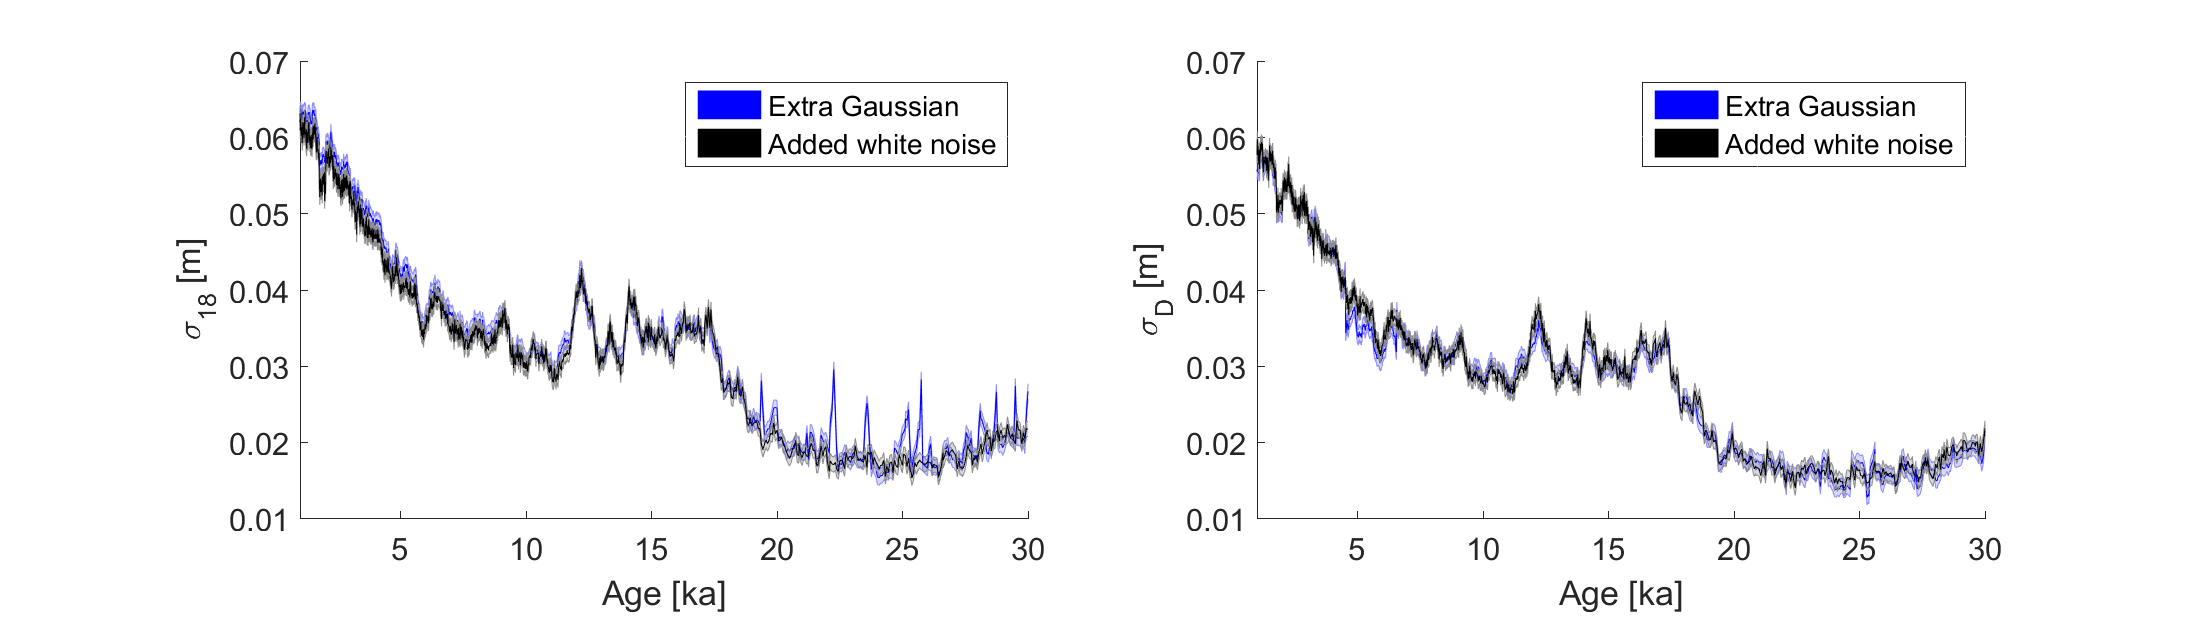
\includegraphics[width=\linewidth]{WAIS_diffusion_adding_noise.eps}
	\caption{WDC diffusion lengths of $\delta^{18}$O (left) and $\delta$D (right).
		The method that has an extra Gaussian is represented by the blue curve and
		the addition of white noise is represented by the black curve.} \label{WAIS_diffusion_adding_noise}
\end{figure}

\begin{figure}
	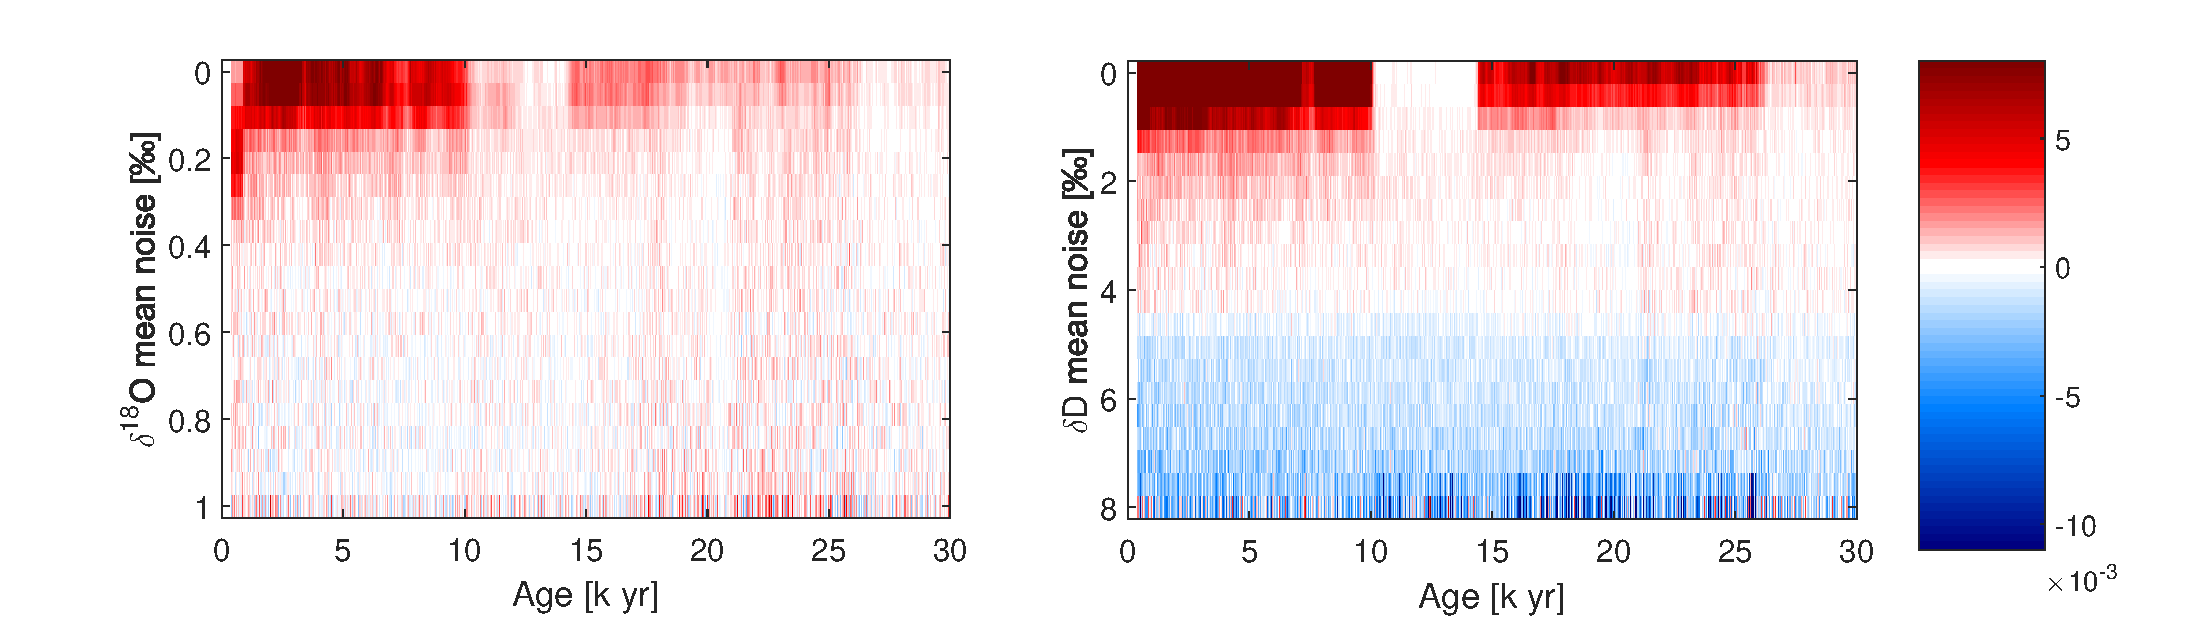
\includegraphics[width=\linewidth]{added_noise_sensitivity.eps}
	\caption{Gradient in estimated diffusion lengths with respect to noise level and age.} \label{added_noise_sensitivity}
\end{figure}

\begin{figure}
	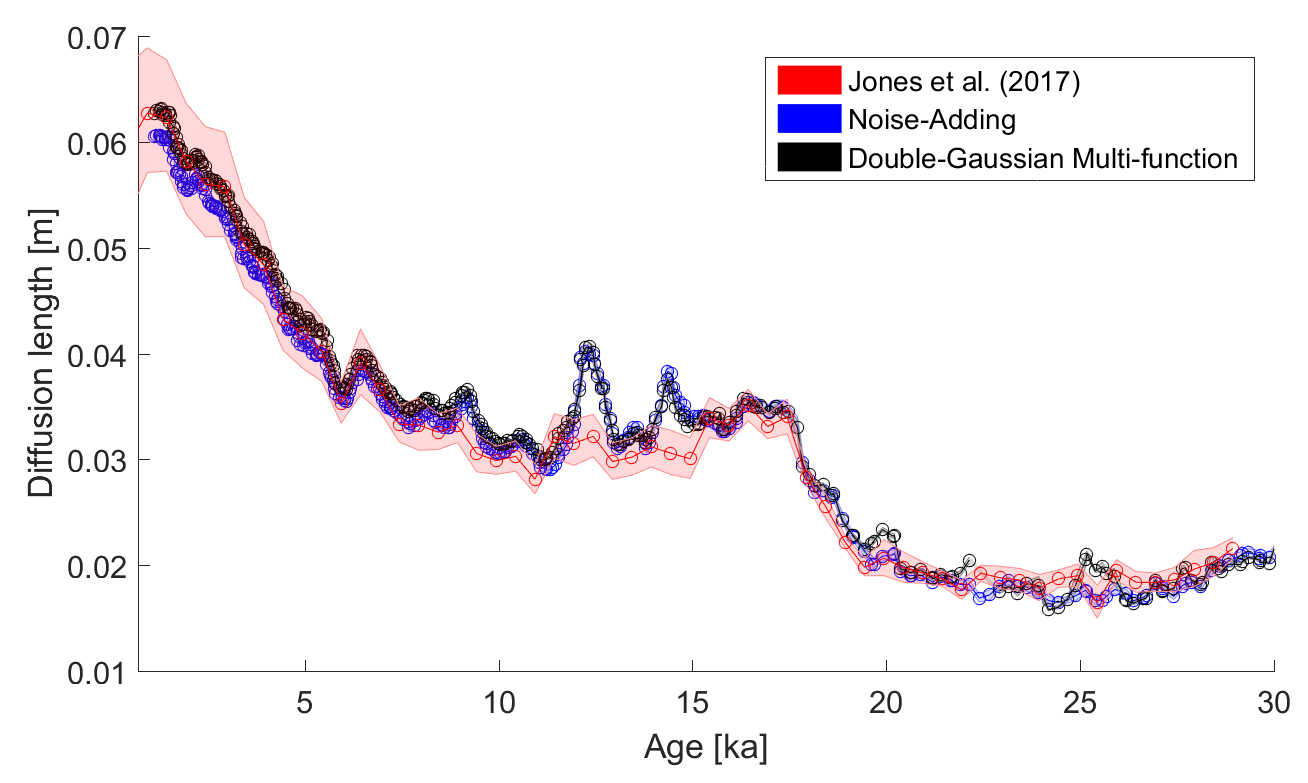
\includegraphics[width=.9\linewidth]{WAIS_diffusion_lengths.eps}
	\caption{Estimated WDC diffusion lengths of $\delta$D compared with \cite{Jones2016}} \label{WAIS_diffusion_lengths}
\end{figure}

\begin{figure}
	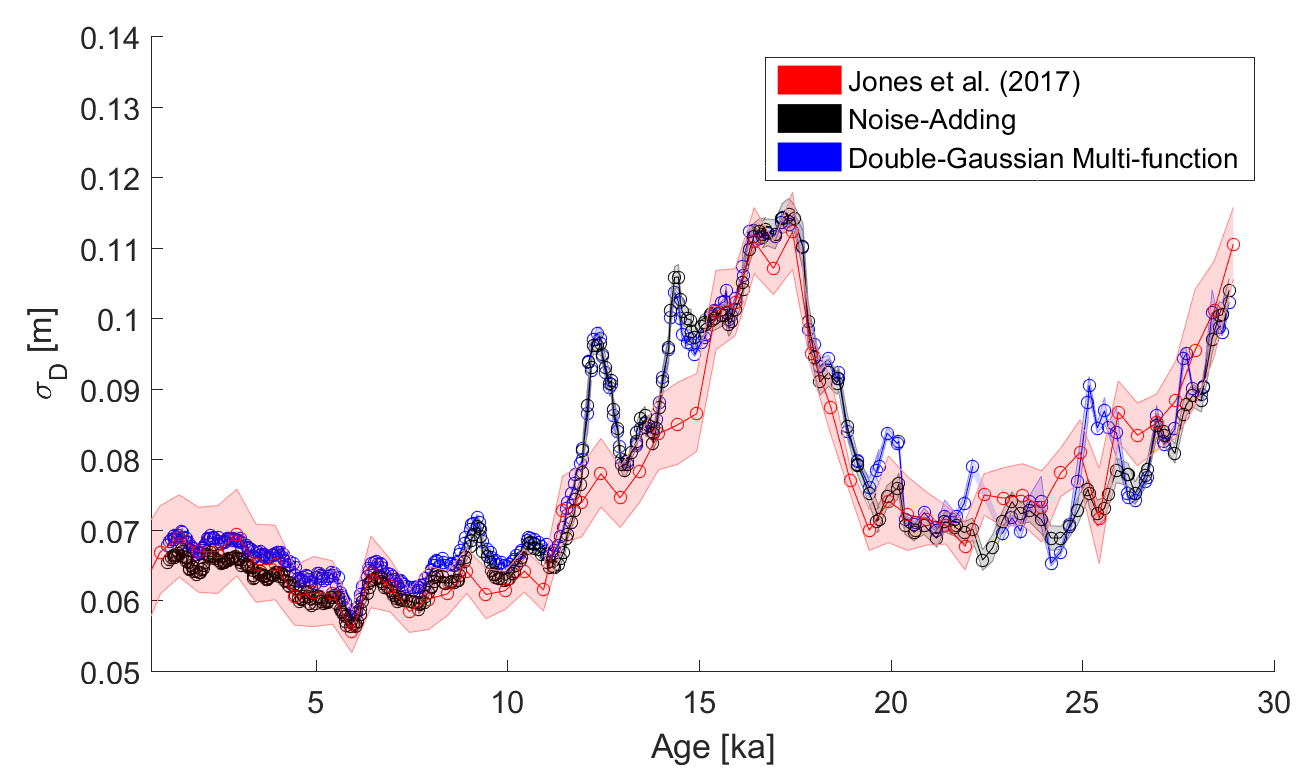
\includegraphics[width=.9\linewidth]{WAIS_diffusion_lengths_thinning_corr.eps}
	\caption{Thinning corrected WDC diffusion lengths compared of $\delta$D with \cite{Jones2016}} \label{WAIS_diffusion_lengths_thinning_corr}
\end{figure}




\begin{figure}
	\sidebyside
	{
		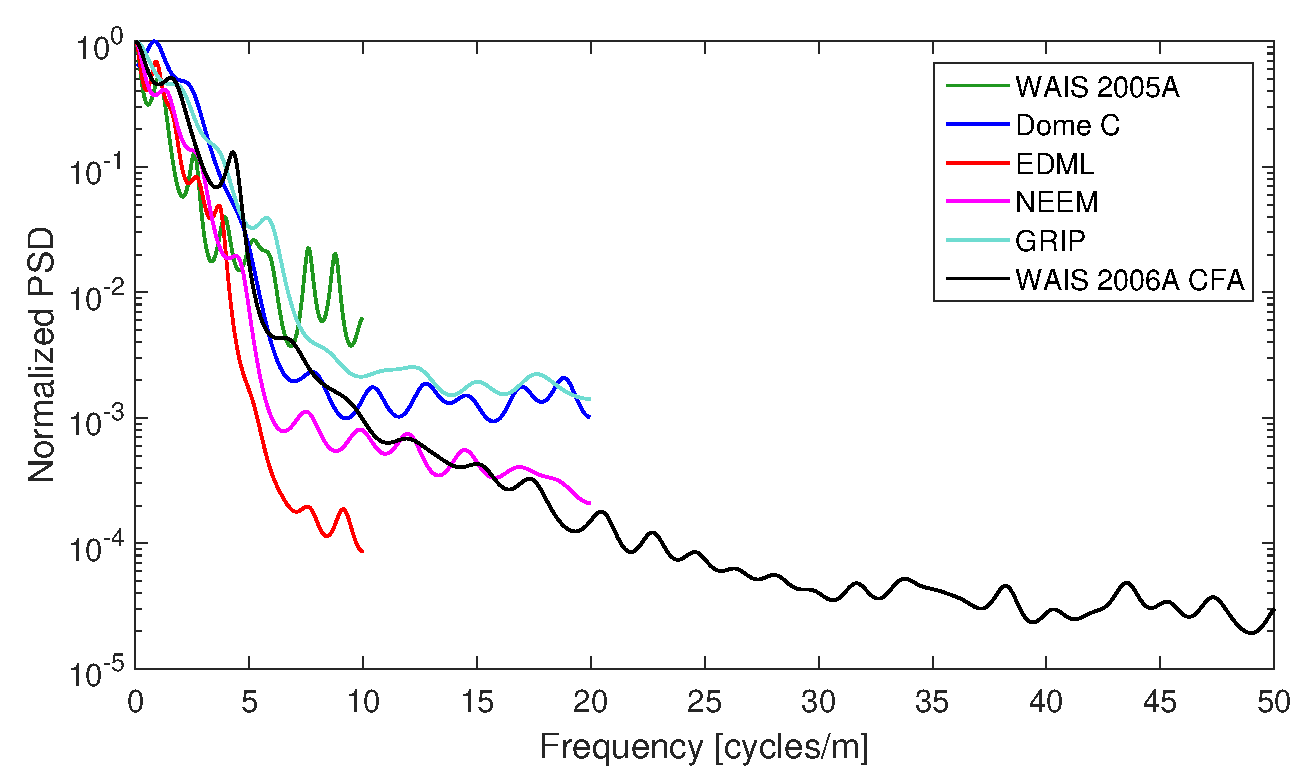
\includegraphics[width=.5\linewidth]{PSD_discrete_plus_cfa_v1.eps}
		\caption{The normalized PSD of five discretely measured $\delta^{18}\mathrm{O}$ series plotted together with the PSD of a $\delta^{18}\mathrm{O}$ WDC section.}\label{spectra_disVScfa}
	}
	{
			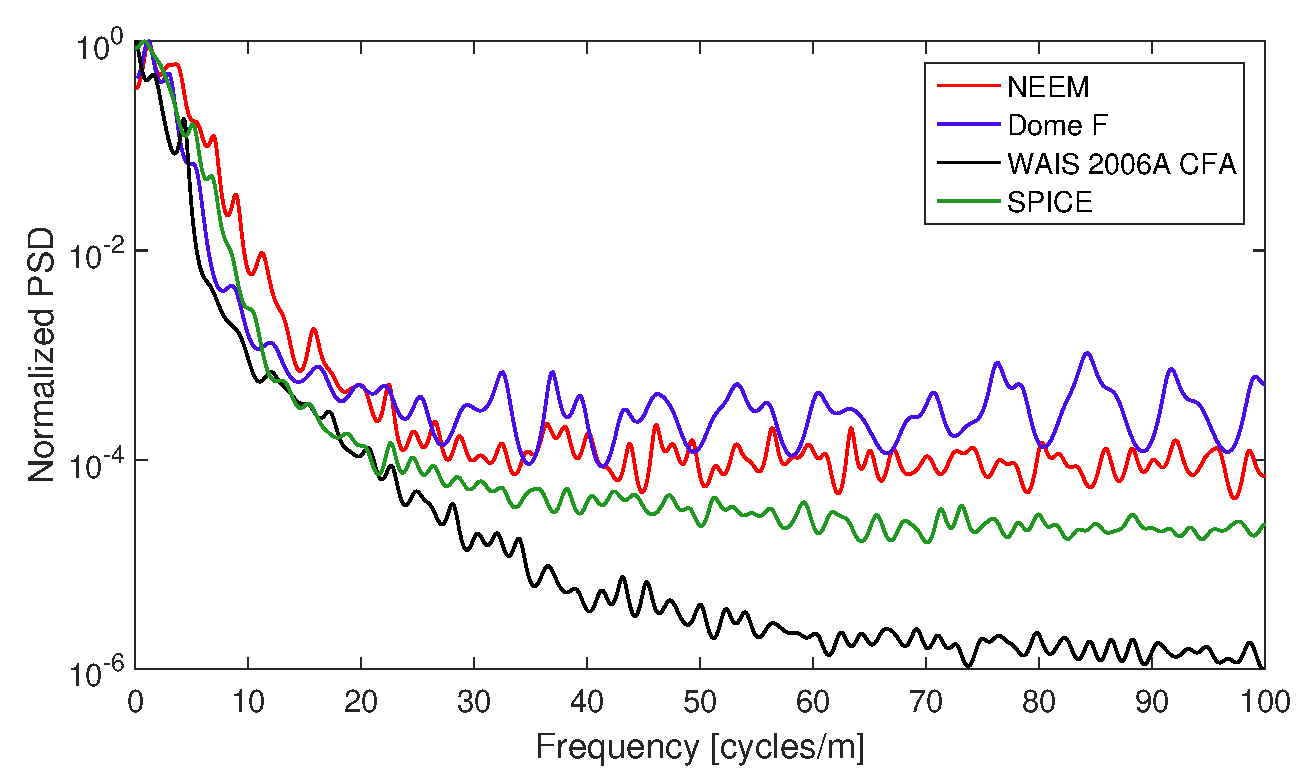
\includegraphics[width=.5\linewidth]{PSD_CFA_v1.eps}
		\caption{The normalized PSD of four continiouysly measured $\delta$D series.}\label{PSD_CFA_v1}
	}
\end{figure}
........................

\begin{figure}
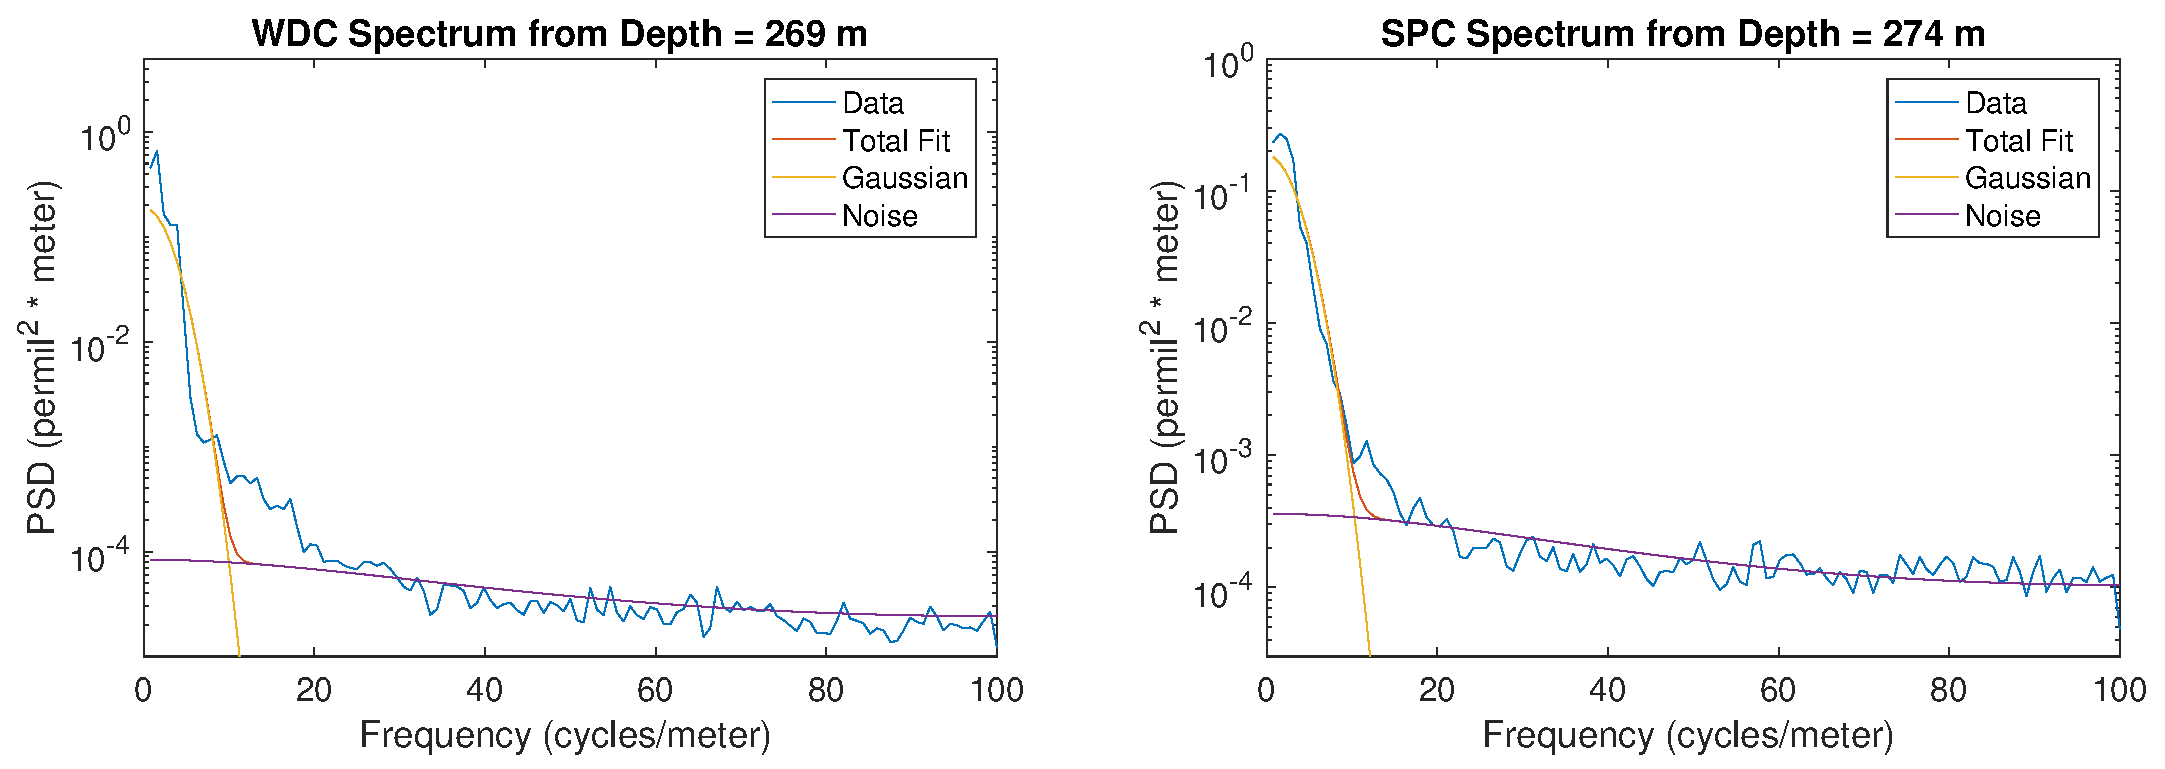
\includegraphics[width=.9\linewidth]{1_gauss.eps}
\caption{WDC and SPC spectra fits with single-Gaussian multi-function technique}\label{1_gauss}
\end{figure}

\begin{figure}
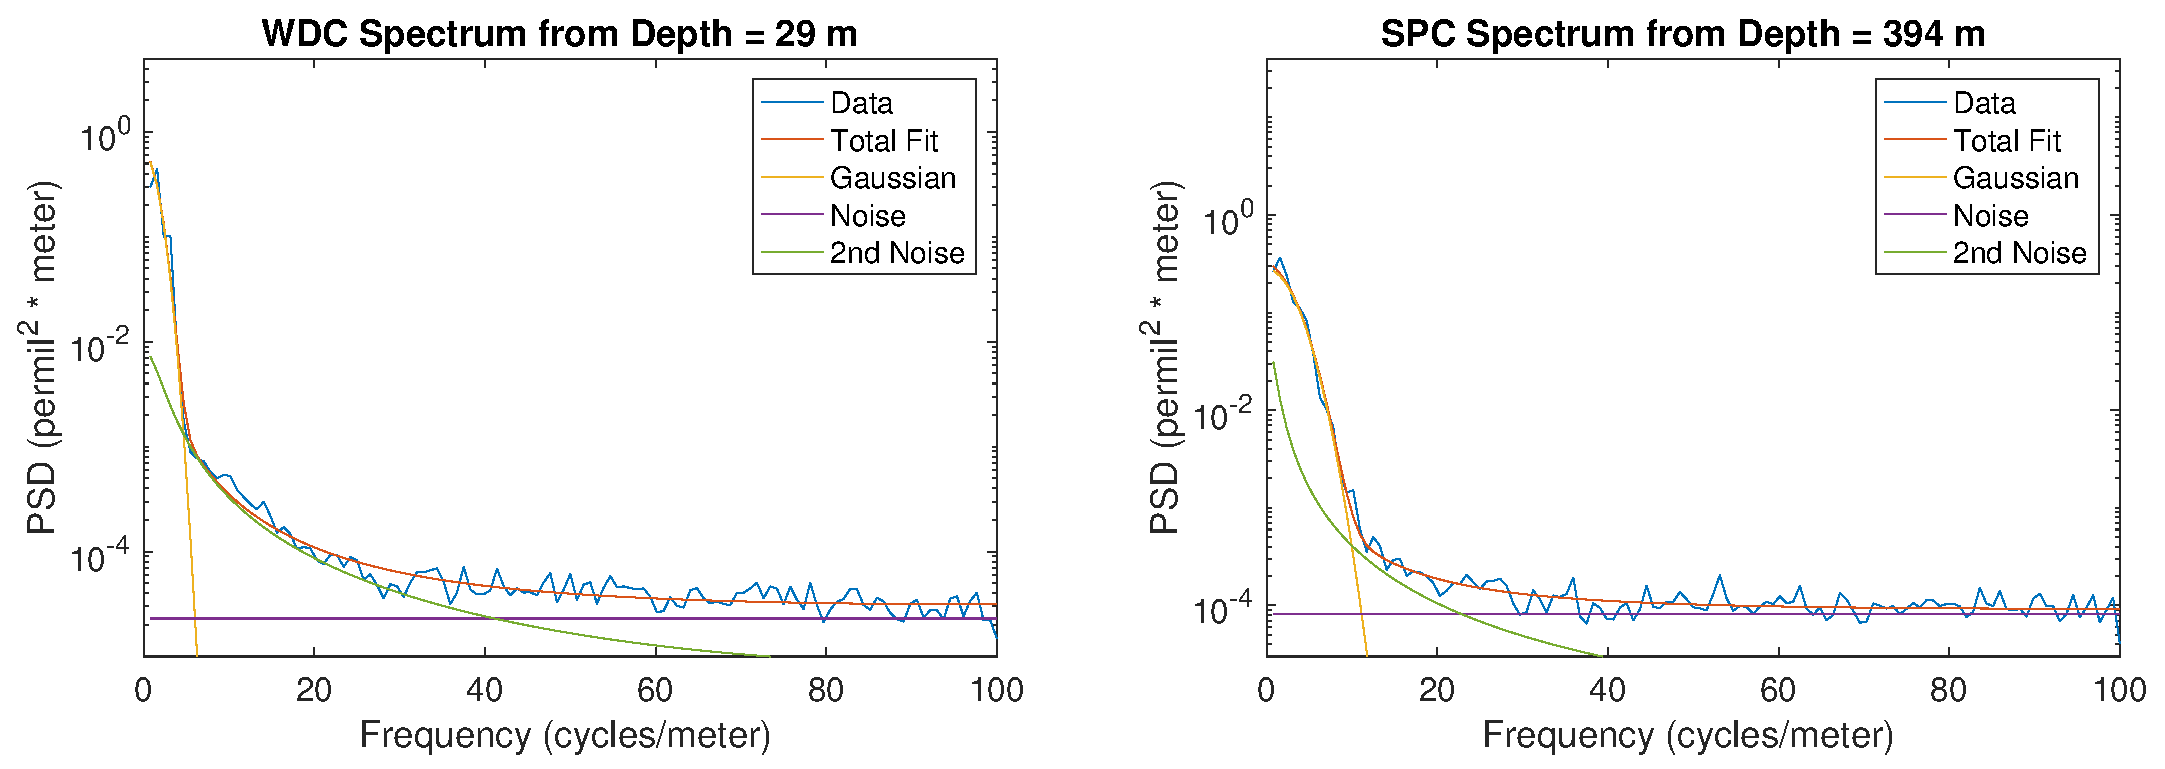
\includegraphics[width=.9\linewidth]{GRR_fit.eps}
\caption{WDC and SPC spectra fits with a single Gaussian and two autoregressive noise functions}\label{GRR_fit}
\end{figure}

\begin{figure}
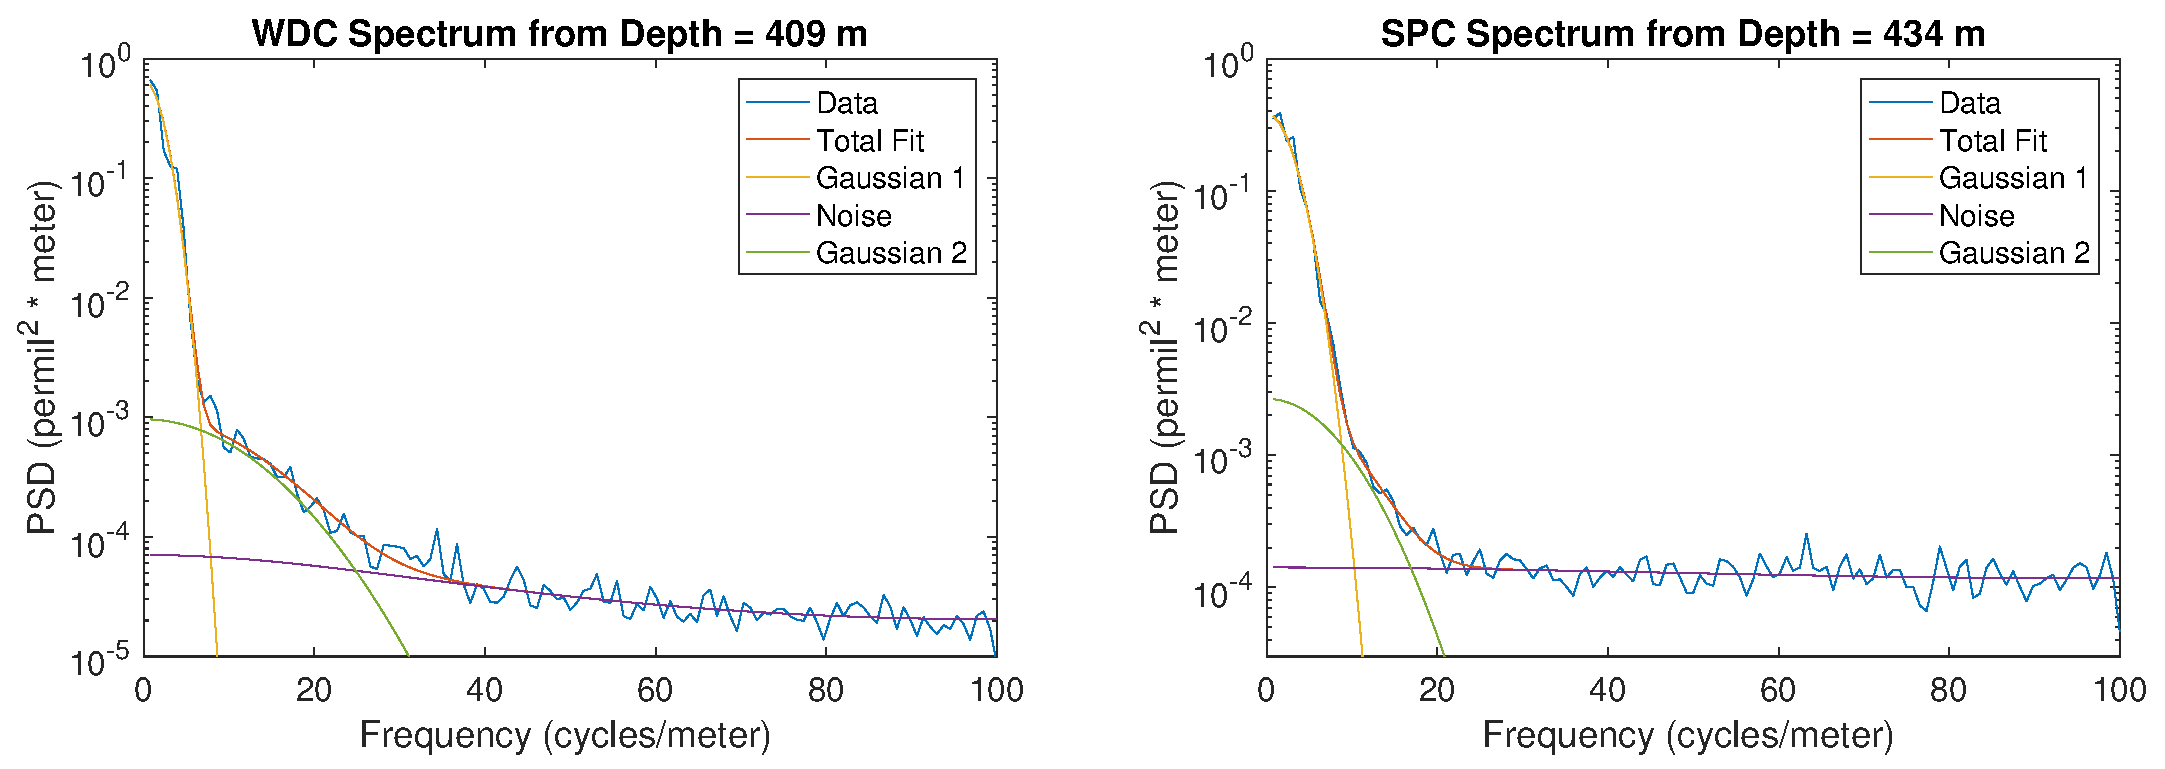
\includegraphics[width=.9\linewidth]{2_gauss.eps}
\caption{WDC and SPC spectra fits with double-Gaussian multi-function technique}\label{2_gauss}
\end{figure}

\begin{figure}
	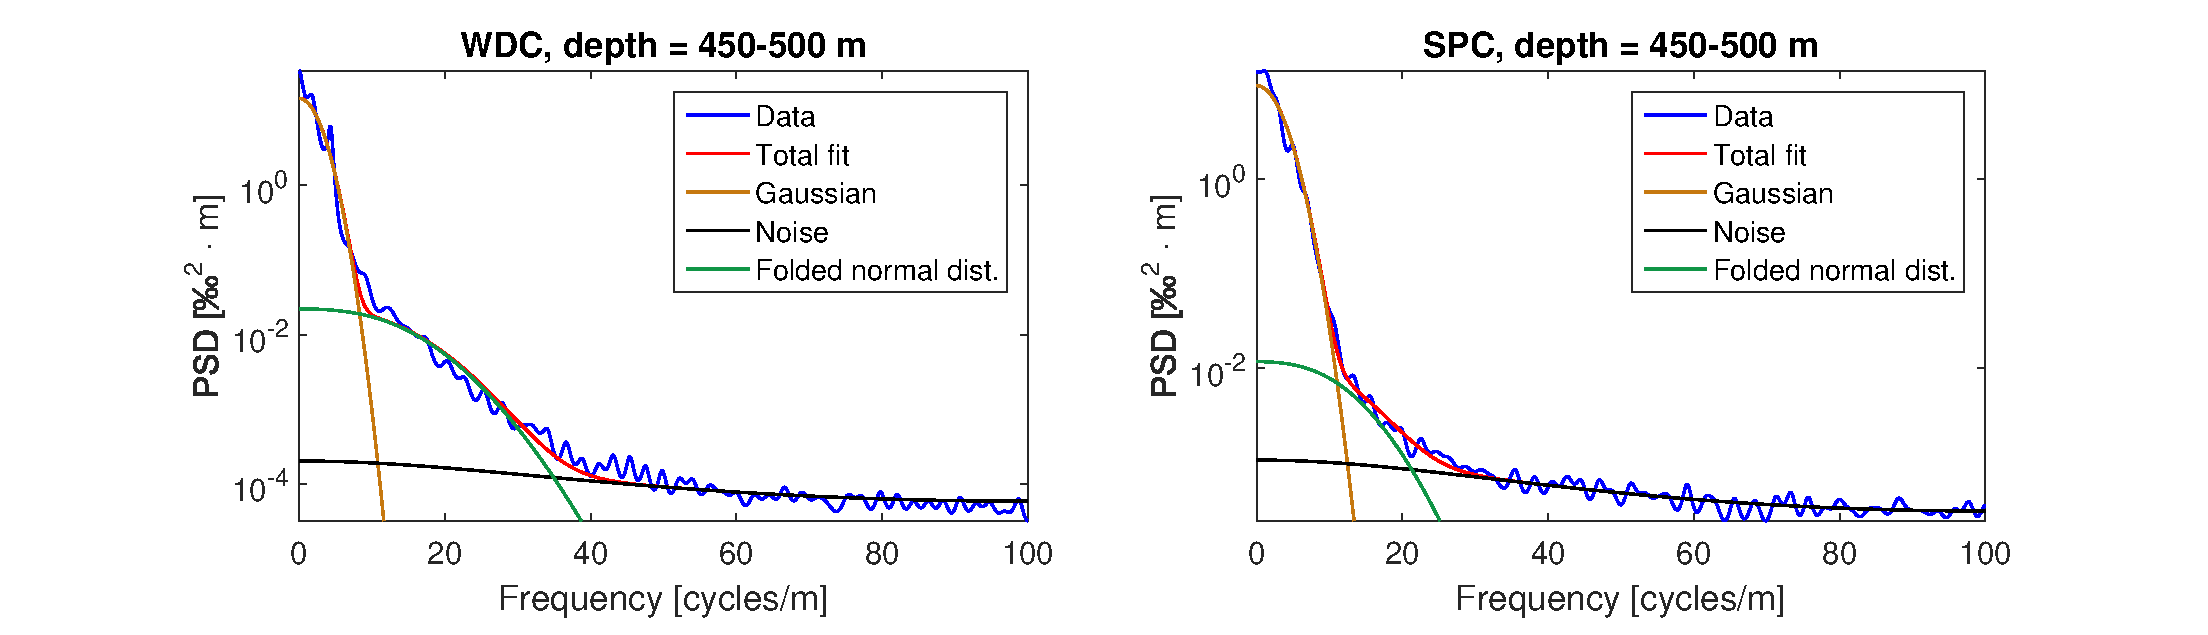
\includegraphics[width=1.1\linewidth]{folded_normal_gauss_spectrum.eps}
	\caption{WDC and SPC spectra fits with double-Gaussian multi-function technique}\label{folded_normal_gauss_spectrum}
\end{figure}


\begin{figure}
\includegraphics[width=.9\linewidth]{sigma_comp.eps}
\caption{Comparison of diffusion length $\sigma$ as calculated by cut-off technique and multi-function technique (single and double Gaussian) for WDC and SPC}\label{sigma_comp}
\end{figure}

\begin{figure}
	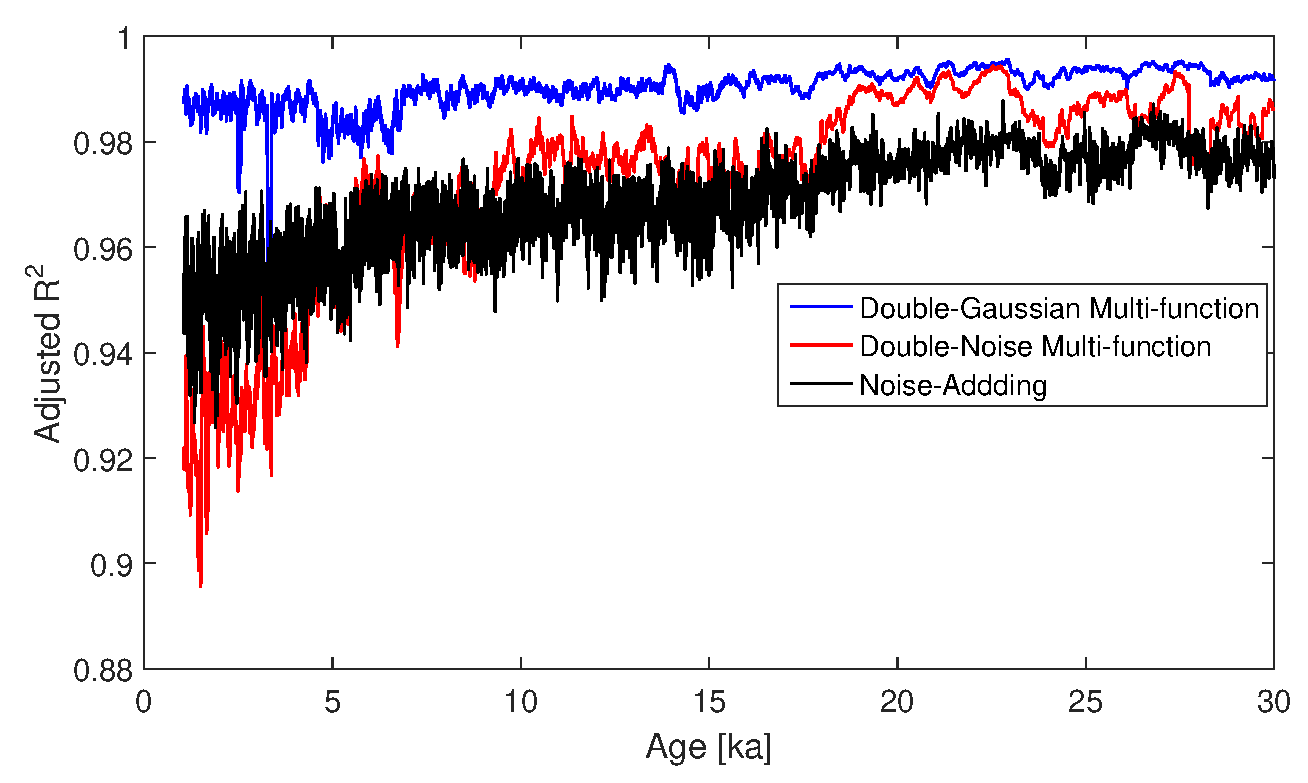
\includegraphics[width=.9\linewidth]{G_of_fit_1.eps}
	\caption{The adjusted goodness of fit calculations through age. } \label{G_of_fit_1}
\end{figure}

\begin{figure}
	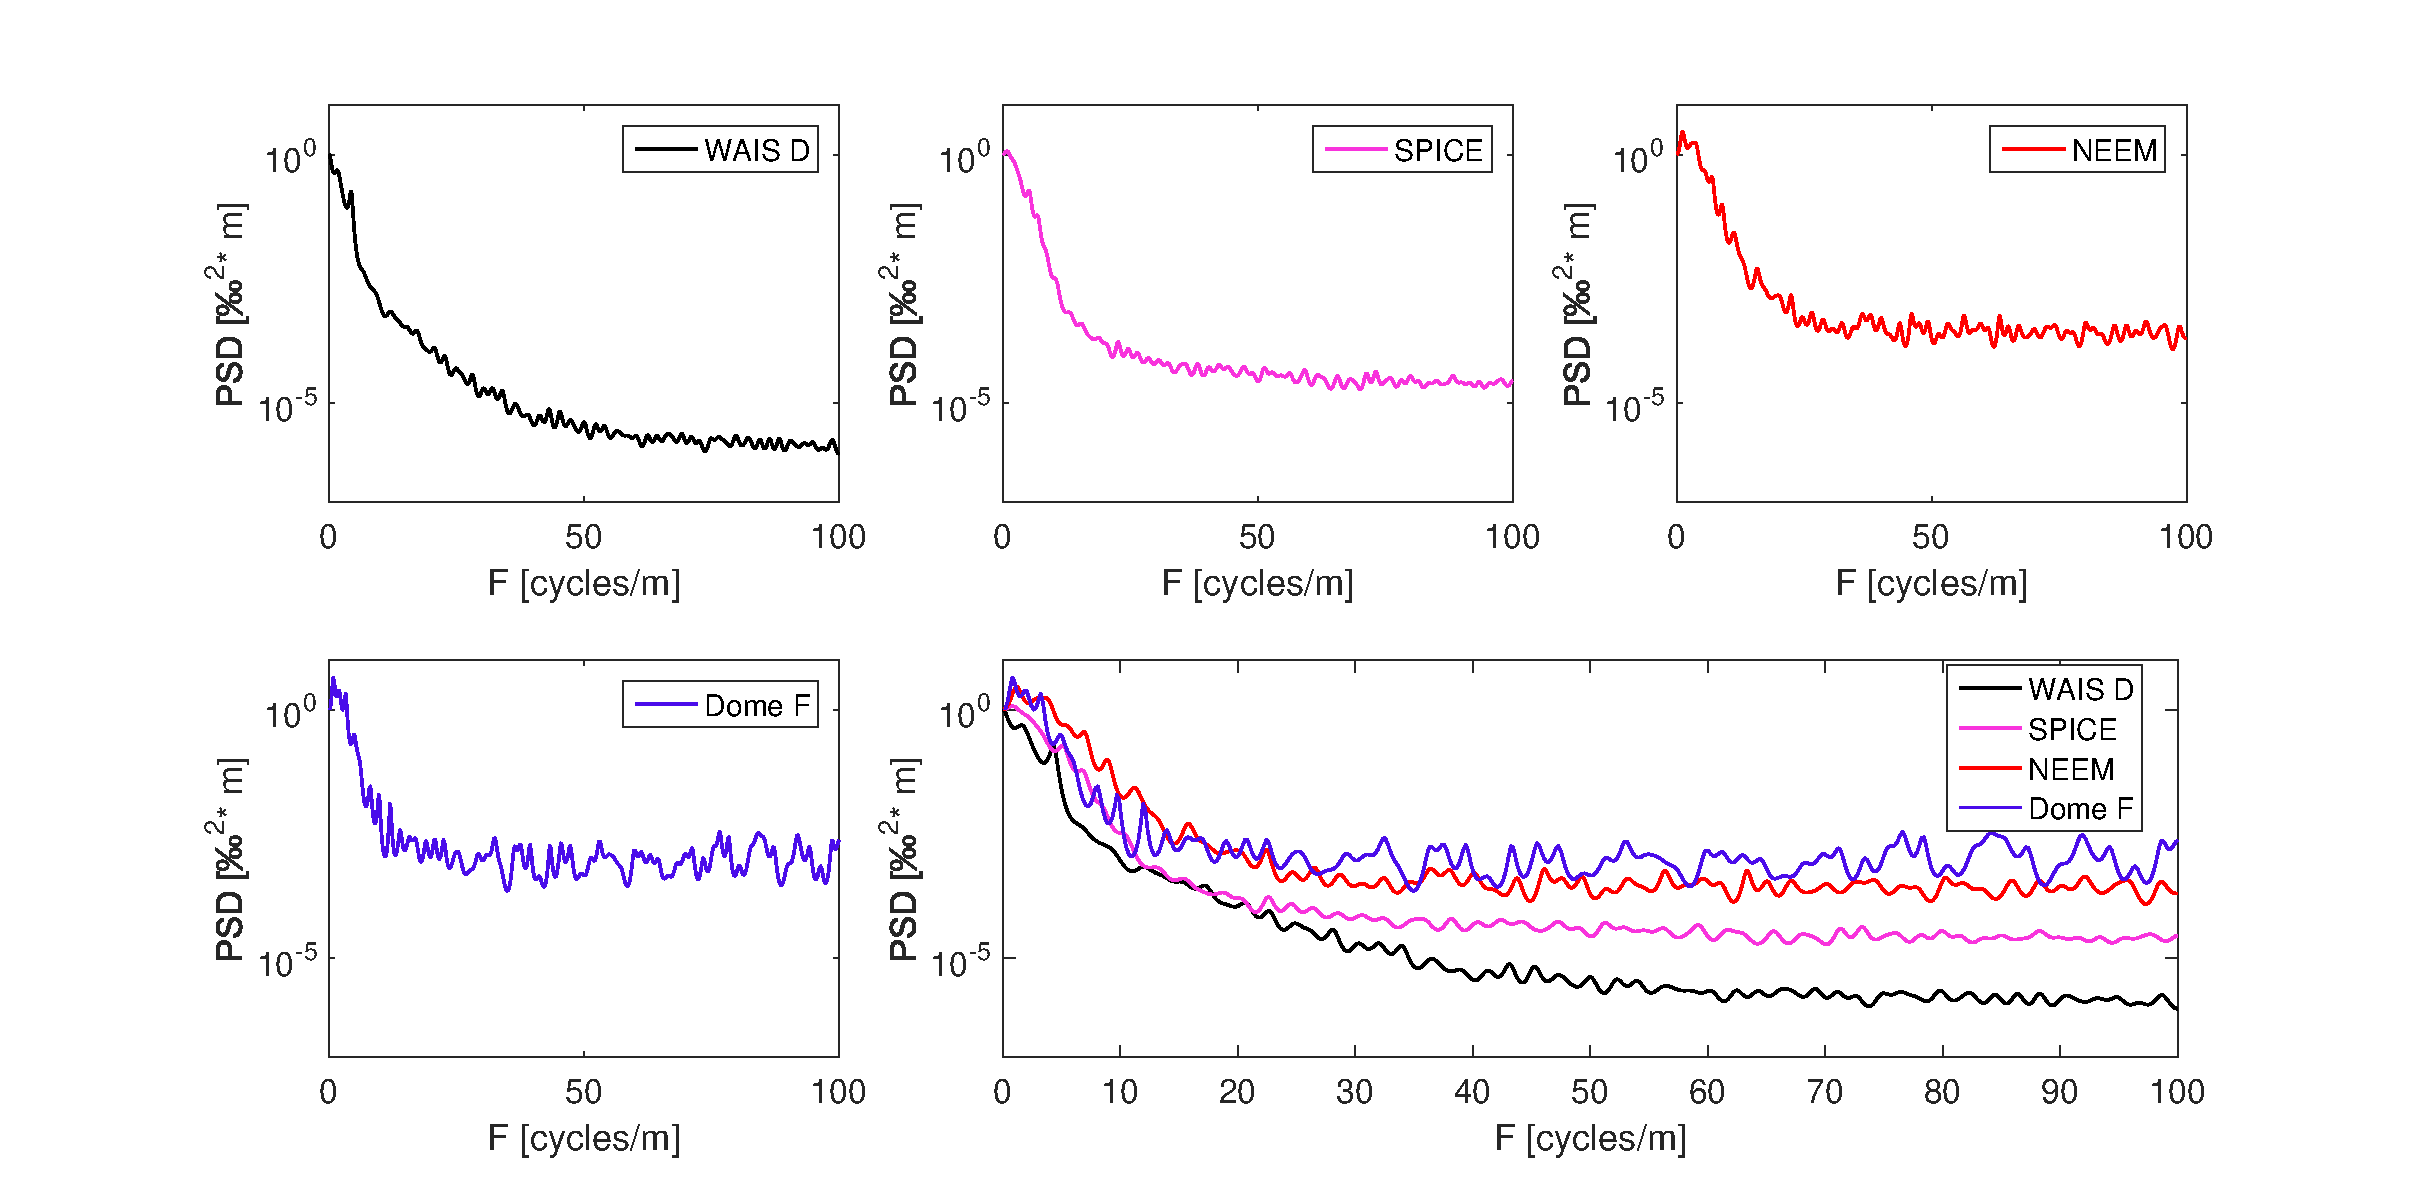
\includegraphics[width=.9\linewidth]{CFA_spectra.eps}
	\caption{Normalized power spectral densities of $\delta$D records measured with different CFA systems. } \label{CFA_spectra}
\end{figure}

\begin{figure}
	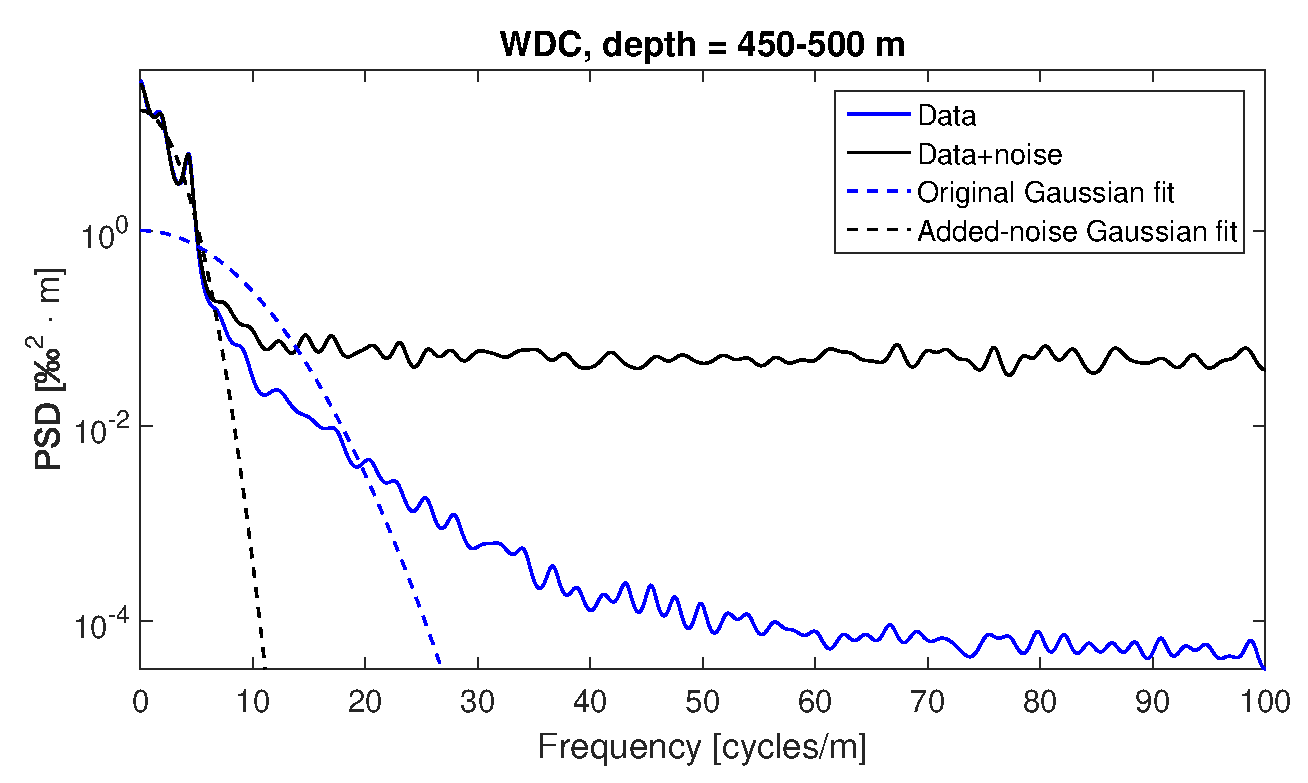
\includegraphics[width=.9\linewidth]{WAIS_spectrum_added_noise.eps}
	\caption{PSD of $\delta$D for a WDC section (solid curves). Blue curve represents
		the measured signal and the black curve represents the modified signal.
		The dashed lines represent the fitted Gaussian function which
		corresponds to the firn diffusion.} \label{WAIS_spectrum_added_noise}
\end{figure}

\begin{figure}
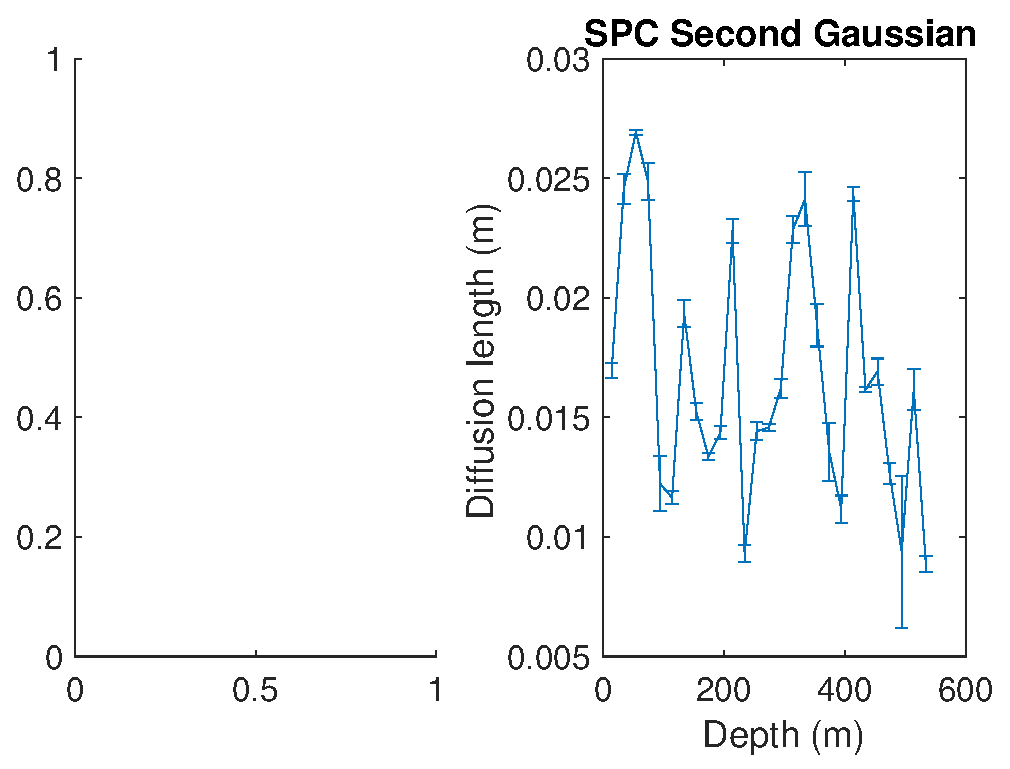
\includegraphics[width=.9\linewidth]{sigma2.eps}
\caption{Plot the $\sigma$ from the second Gaussian for WDC and SPC}\label{sigma2}
\end{figure}

\begin{figure}
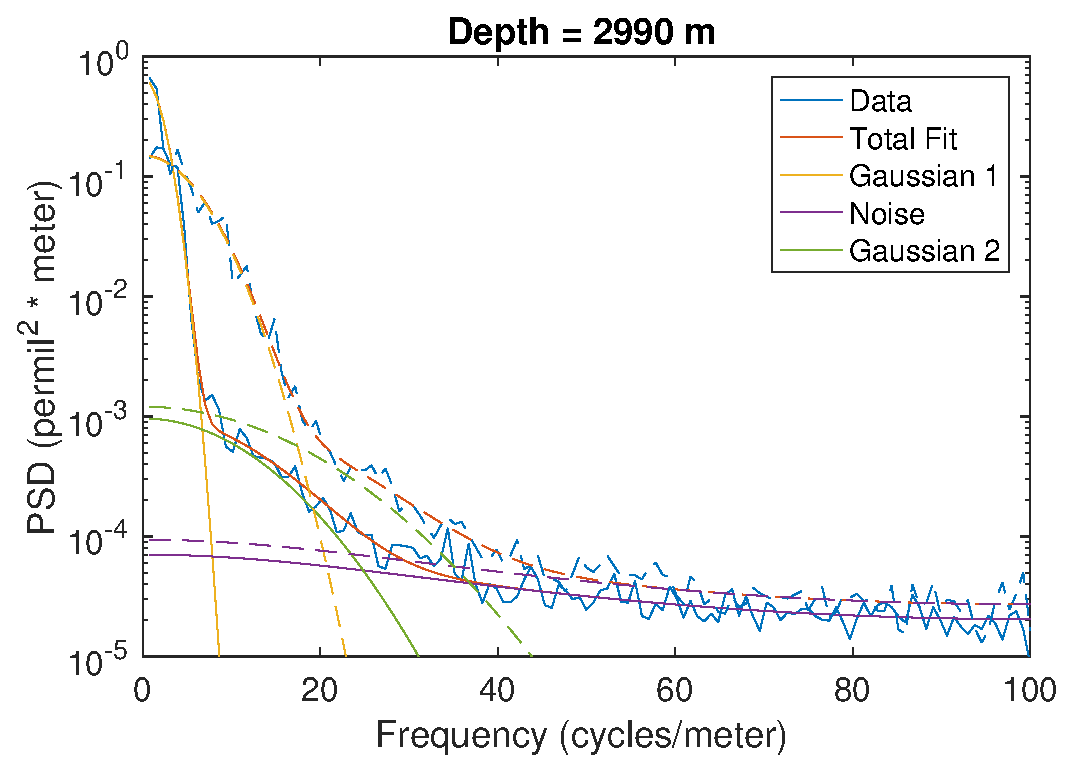
\includegraphics[width=.9\linewidth]{sigmadependence.eps}
\caption{Showing how sigma2 depends on sigma1}\label{sigmadependence}
\end{figure}

\begin{figure}
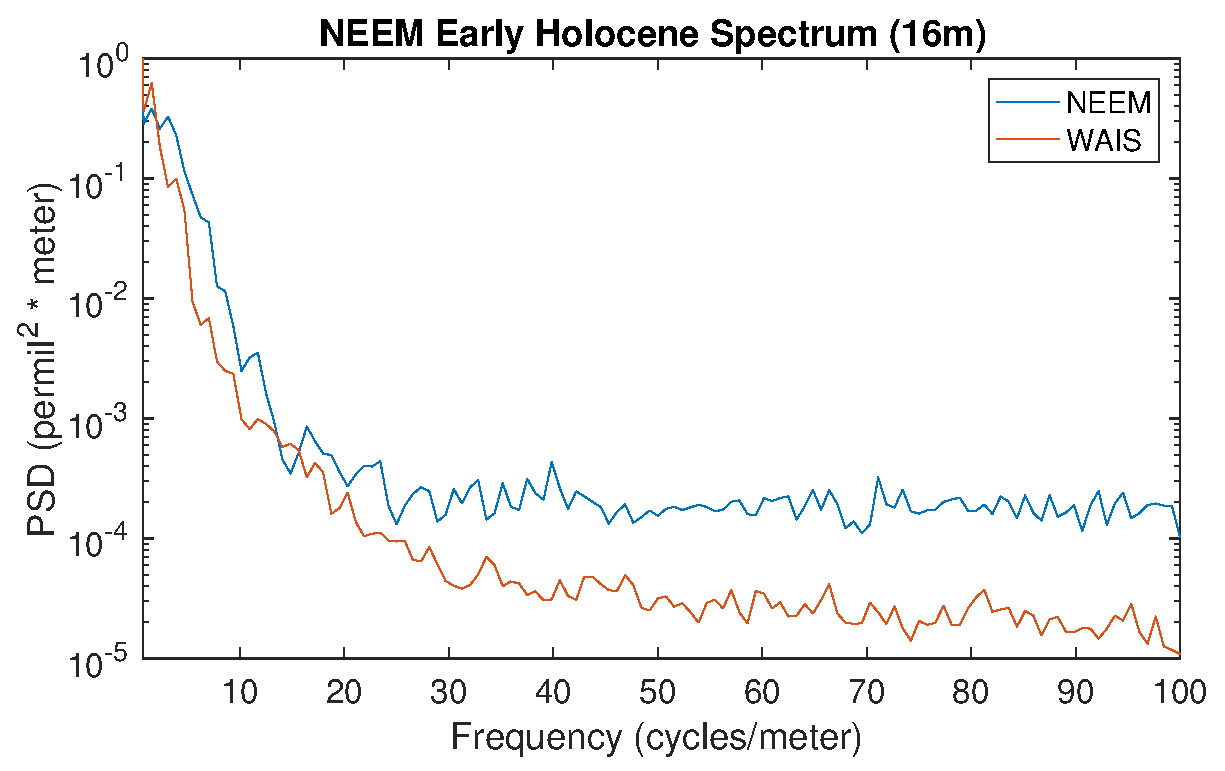
\includegraphics[width=.9\linewidth]{NEEMspec.eps}
\caption{Spectra from NEEM 1382-1398 meters, CFA data measured on a different system}\label{NEEMspec}
\end{figure}

\begin{table}
\caption{Placeholder table}\label{sampletable}
\begin{tabular}{l l l}
\hline
\textbf{Treatments} & \textbf{Response 1} & \textbf{Response 2}\\
\hline
Treatment 1 & 0.0003262 & 0.562 \\
Treatment 2 & 0.0015681 & 0.910 \\
Treatment 3 & 0.0009271 & 0.296 \\
\hline
\end{tabular}
\end{table}

\end{document}

%%%%%%%%%%%%%%%%%%%%%%%%%%%%%%%%%%%%%%%%%%%%%%%%%%%%%%%%%%%%%%%

More Information and Advice:

%% ------------------------------------------------------------------------ %%
%
%  SECTION HEADS
%
%% ------------------------------------------------------------------------ %%

% Capitalize the first letter of each word (except for
% prepositions, conjunctions, and articles that are
% three or fewer letters).

% AGU follows standard outline style; therefore, there cannot be a section 1 without
% a section 2, or a section 2.3.1 without a section 2.3.2.
% Please make sure your section numbers are balanced.
% ---------------
% Level 1 head
%
% Use the \section{} command to identify level 1 heads;
% type the appropriate head wording between the curly
% brackets, as shown below.
%
%An example:
%\section{Level 1 Head: Introduction}
%
% ---------------
% Level 2 head
%
% Use the \subsection{} command to identify level 2 heads.
%An example:
%\subsection{Level 2 Head}
%
% ---------------
% Level 3 head
%
% Use the \subsubsection{} command to identify level 3 heads
%An example:
%\subsubsection{Level 3 Head}
%
%---------------
% Level 4 head
%
% Use the \subsubsubsection{} command to identify level 3 heads
% An example:
%\subsubsubsection{Level 4 Head} An example.
%
%% ------------------------------------------------------------------------ %%
%
%  IN-TEXT LISTS
%
%% ------------------------------------------------------------------------ %%
%
% Do not use bulleted lists; enumerated lists are okay.
% \begin{enumerate}
% \item
% \item
% \item
% \end{enumerate}
%
%% ------------------------------------------------------------------------ %%
%
%  EQUATIONS
%
%% ------------------------------------------------------------------------ %%

% Single-line equations are centered.
% Equation arrays will appear left-aligned.

Math coded inside display math mode \[ ...\]
 will not be numbered, e.g.,:
 \[ x^2=y^2 + z^2\]

 Math coded inside \begin{equation} and \end{equation} will
 be automatically numbered, e.g.,:
 \begin{equation}
 x^2=y^2 + z^2
 \end{equation}

% IF YOU HAVE MULTI-LINE EQUATIONS, PLEASE
% BREAK THE EQUATIONS INTO TWO OR MORE LINES
% OF SINGLE COLUMN WIDTH (20 pc, 8.3 cm)
% using double backslashes (\\).

% To create multiline equations, use the
% \begin{eqnarray} and \end{eqnarray} environment
% as demonstrated below.
\begin{eqnarray}
  x_{1} & = & (x - x_{0}) \cos \Theta \nonumber \\
        && + (y - y_{0}) \sin \Theta  \nonumber \\
  y_{1} & = & -(x - x_{0}) \sin \Theta \nonumber \\
        && + (y - y_{0}) \cos \Theta.
\end{eqnarray}

%If you don't want an equation number, use the star form:
%\begin{eqnarray*}...\end{eqnarray*}

% Break each line at a sign of operation
% (+, -, etc.) if possible, with the sign of operation
% on the new line.

% Indent second and subsequent lines to align with the first character following the equal sign on the first line.

% Use an \hspace{} command to insert horizontal space into your equation if necessary. Place an appropriate unit of measure between the curly braces, e.g. \hspace{1in}; you may have to experiment to achieve the correct amount of space.


%% ------------------------------------------------------------------------ %%
%
%  EQUATION NUMBERING: COUNTER
%
%% ------------------------------------------------------------------------ %%

% You may change equation numbering by resetting
% the equation counter or by explicitly numbering
% an equation.

% To explicitly number an equation, type \eqnum{}
% (with the desired number between the brackets)
% after the \begin{equation} or \begin{eqnarray}
% command.  The \eqnum{} command will affect only
% the equation it appears with; LaTeX will number
% any equations appearing later in the manuscript
% according to the equation counter.
%

% If you have a multiline equation that needs only
% one equation number, use a \nonumber command in
% front of the double backslashes (\\) as shown in
% the multiline equation above.

%% ------------------------------------------------------------------------ %%
%
%  SIDEWAYS FIGURE AND TABLE EXAMPLES
%
%% ------------------------------------------------------------------------ %%
%
% For tables and figures, add \usepackage{rotating} to the paper and add the rotating.sty file to the folder.
% AGU prefers the use of {sidewaystable} over {landscapetable} as it causes fewer problems.
%
% \begin{sidewaysfigure}
% \includegraphics[width=20pc]{samplefigure.eps}
% \caption{caption here}
% \label{label_here}
% \end{sidewaysfigure}
%
% \begin{sidewaystable}
% \caption{}
% \begin{tabular}
% Table layout here.
% \end{tabular}
% \end{sidewaystable}
